\chapter{Trabajo realizado} \label{TrabajoTT2}
En este capítulo se habla de los \textit{sprints} de la etapa de producción que
abarcan el trabajo terminal 2, es decir los \textit{sprints} del tres al diez. El
onceavo \textit{sprint} no es abarcado en este capítulo ya que de él se habla en la
sección correspondiente a la pruebas. Cada \textit{sprint} es abordado mencionando
primeramente su objetivo, después se describe todo lo realizado durante el
\textit{sprint} y se finaliza mencionando si se completo el \textit{sprint} y que
se obtuvo al final del mismo. Es importante recalcar que los \textit{sprints} se
abordan en este capítulo de manera secuencial, sin embargo los \textit{sprints}
impares corresponden al desarrollo de los niveles impares, mientras que los pares
corresponden al desarrollo de los niveles pares; esto debido a la nueva asignación
de trabajo, ver sección \ref{Sec:AsignacionTrabajo}.

%\subsection{Detalles del proyecto}
Aquí se mostrará del proyecto el título, estudio, género, plataforma, fecha de inicio, fecha de término, lo planeado, en desarrollo, sin planear y terminado.
\\
\subsubsection{Título}
Yolotl

\subsubsection{Estudio}
ESCOM - IPN

\subsubsection{Plataforma}
Dispositivos móviles android

\subsubsection{Fecha de inicio}
1 Agosto 2017

\subsubsection{Fecha de término}
1 Junio 2018
\subsubsection{Planeado}
El 80\%
\subsubsection{Desarrollo}
El 10\%
\subsubsection{Planear}
El 20\%
\subsubsection{Terminado}
El 0\%



\subsection{Sprint plan 1}
\subsubsection{SprintID}
01
\subsubsection{Inicio}
1 Agosto 2017
\subsubsection{Fin}
31 Agosto 2017
\subsubsection{Meta}
Nivel 1
\subsubsection{Porcentaje}
El 16\% 


\subsubsection{FeatureID}
01
\subsubsection{Nombre}
N1
\subsubsection{Estado}
Planeado

\subsubsection{SprintID}
01
\subsubsection{Comentarios}
-


\subsection{Sprint backlog 1}
\subsubsection{Sprint backlog}
01

\subsubsection{Tareas}
6
\subsubsection{Tendencia}
0
\subsubsection{Esfuerzo restante}
56
\subsubsection{Tendencia actual}
-
\subsubsection{Progreso ideal}
10
\subsubsection{Tareas restantes}
10
\subsubsection{Nombre de la tarea}
n1
\subsubsection{FeatureID}
01
\subsubsection{Miembro}
Rocío
\subsubsection{Rol}
Desarrollo
\subsubsection{Estado}
Planeado
\subsubsection{Esfuerzo}
10
\subsection{Buglist}
\subsubsection{BugID}
01
\subsubsection{Descripción}
Doble salto infinito
\subsubsection{Descripción técnica}
El gameobject no realiza la función detectar colisión de el "piso" 
\subsubsection{Autor}
Velez
\subsubsection{Estado}
Revisión
\subsubsection{FeatureID}
01


\subsection{Task Slips 1}


\subsubsection{FeatureID}1
\subsubsection{Nombre}Maqueta
\subsubsection{Tarea}Realizar maqueta del nivel completo
\subsubsection{Miembro}Rocío
\subsubsection{Esfuerzo estimado}1
\subsubsection{Terminado}si
\subsubsection{Restante}0


\subsubsection{FeatureID} 1
\subsubsection{Nombre} Enemigos
\subsubsection{Tarea} Realizar el comportamiento de los enemigos o cualquier otra acción necesaria dentro del nivel
\subsubsection{Miembro} Rocio
\subsubsection{Esfuerzo estimado} 3
\subsubsection{Terminado} sí
\subsubsection{Restante} 0


\subsubsection{FeatureID} 1
\subsubsection{Nombre} Arte 1
\subsubsection{Tarea} Crear vista de los personajes
\subsubsection{Miembro} Rocío
\subsubsection{Esfuerzo estimado} 2
\subsubsection{Terminado} sí
\subsubsection{Restante} 0



\subsubsection{FeatureID} 1
\subsubsection{Nombre} Arte 2
\subsubsection{Tarea} Crear el diseño de los obstáculos
\subsubsection{Miembro} Rocío
\subsubsection{Esfuerzo estimado} 2
\subsubsection{Terminado} sí
\subsubsection{Restante} 0


\subsubsection{FeatureID} 1
\subsubsection{Nombre} Arte 3
\subsubsection{Tarea} Crear el diseño de los items
\subsubsection{Miembro} Rocio
\subsubsection{Esfuerzo estimado} 2
\subsubsection{Terminado} sí
\subsubsection{Restante} 0


\section{Tercer sprint de producción}
Esta etapa contiene el desarrollo del nivel tres del juego. El panorama general abarca un nivel de manera ascendente en un terreno rocoso. Después se llega al jefe que tiene forma de jaguar Tepeyóllotl.

Primero se empieza con el maquetado del nivel, para establecer el tamaño del nivel, pues esta vez será de manera vertical el diseño, y la cámara solo se moverá en esa dirección. Se establece también donde debe ir cada objeto o enemigo junto con anotaciones necesarias para la comprensión posterior, como son direcciones de movimiento o acciones que deben realizarse. Aquí se debe tomar muy en cuenta el tamaño del personaje a jugar si no, no se podrá avanzar en el nivel ya que se da la situación a atorarse debido al tamaño, incluido el espacio para saltar. Lo anterior se puede ver en la figura \ref{fig:n01}.
\begin{figure}[htbp]
	\centering
	\subfigure[Primera parte del nivel]{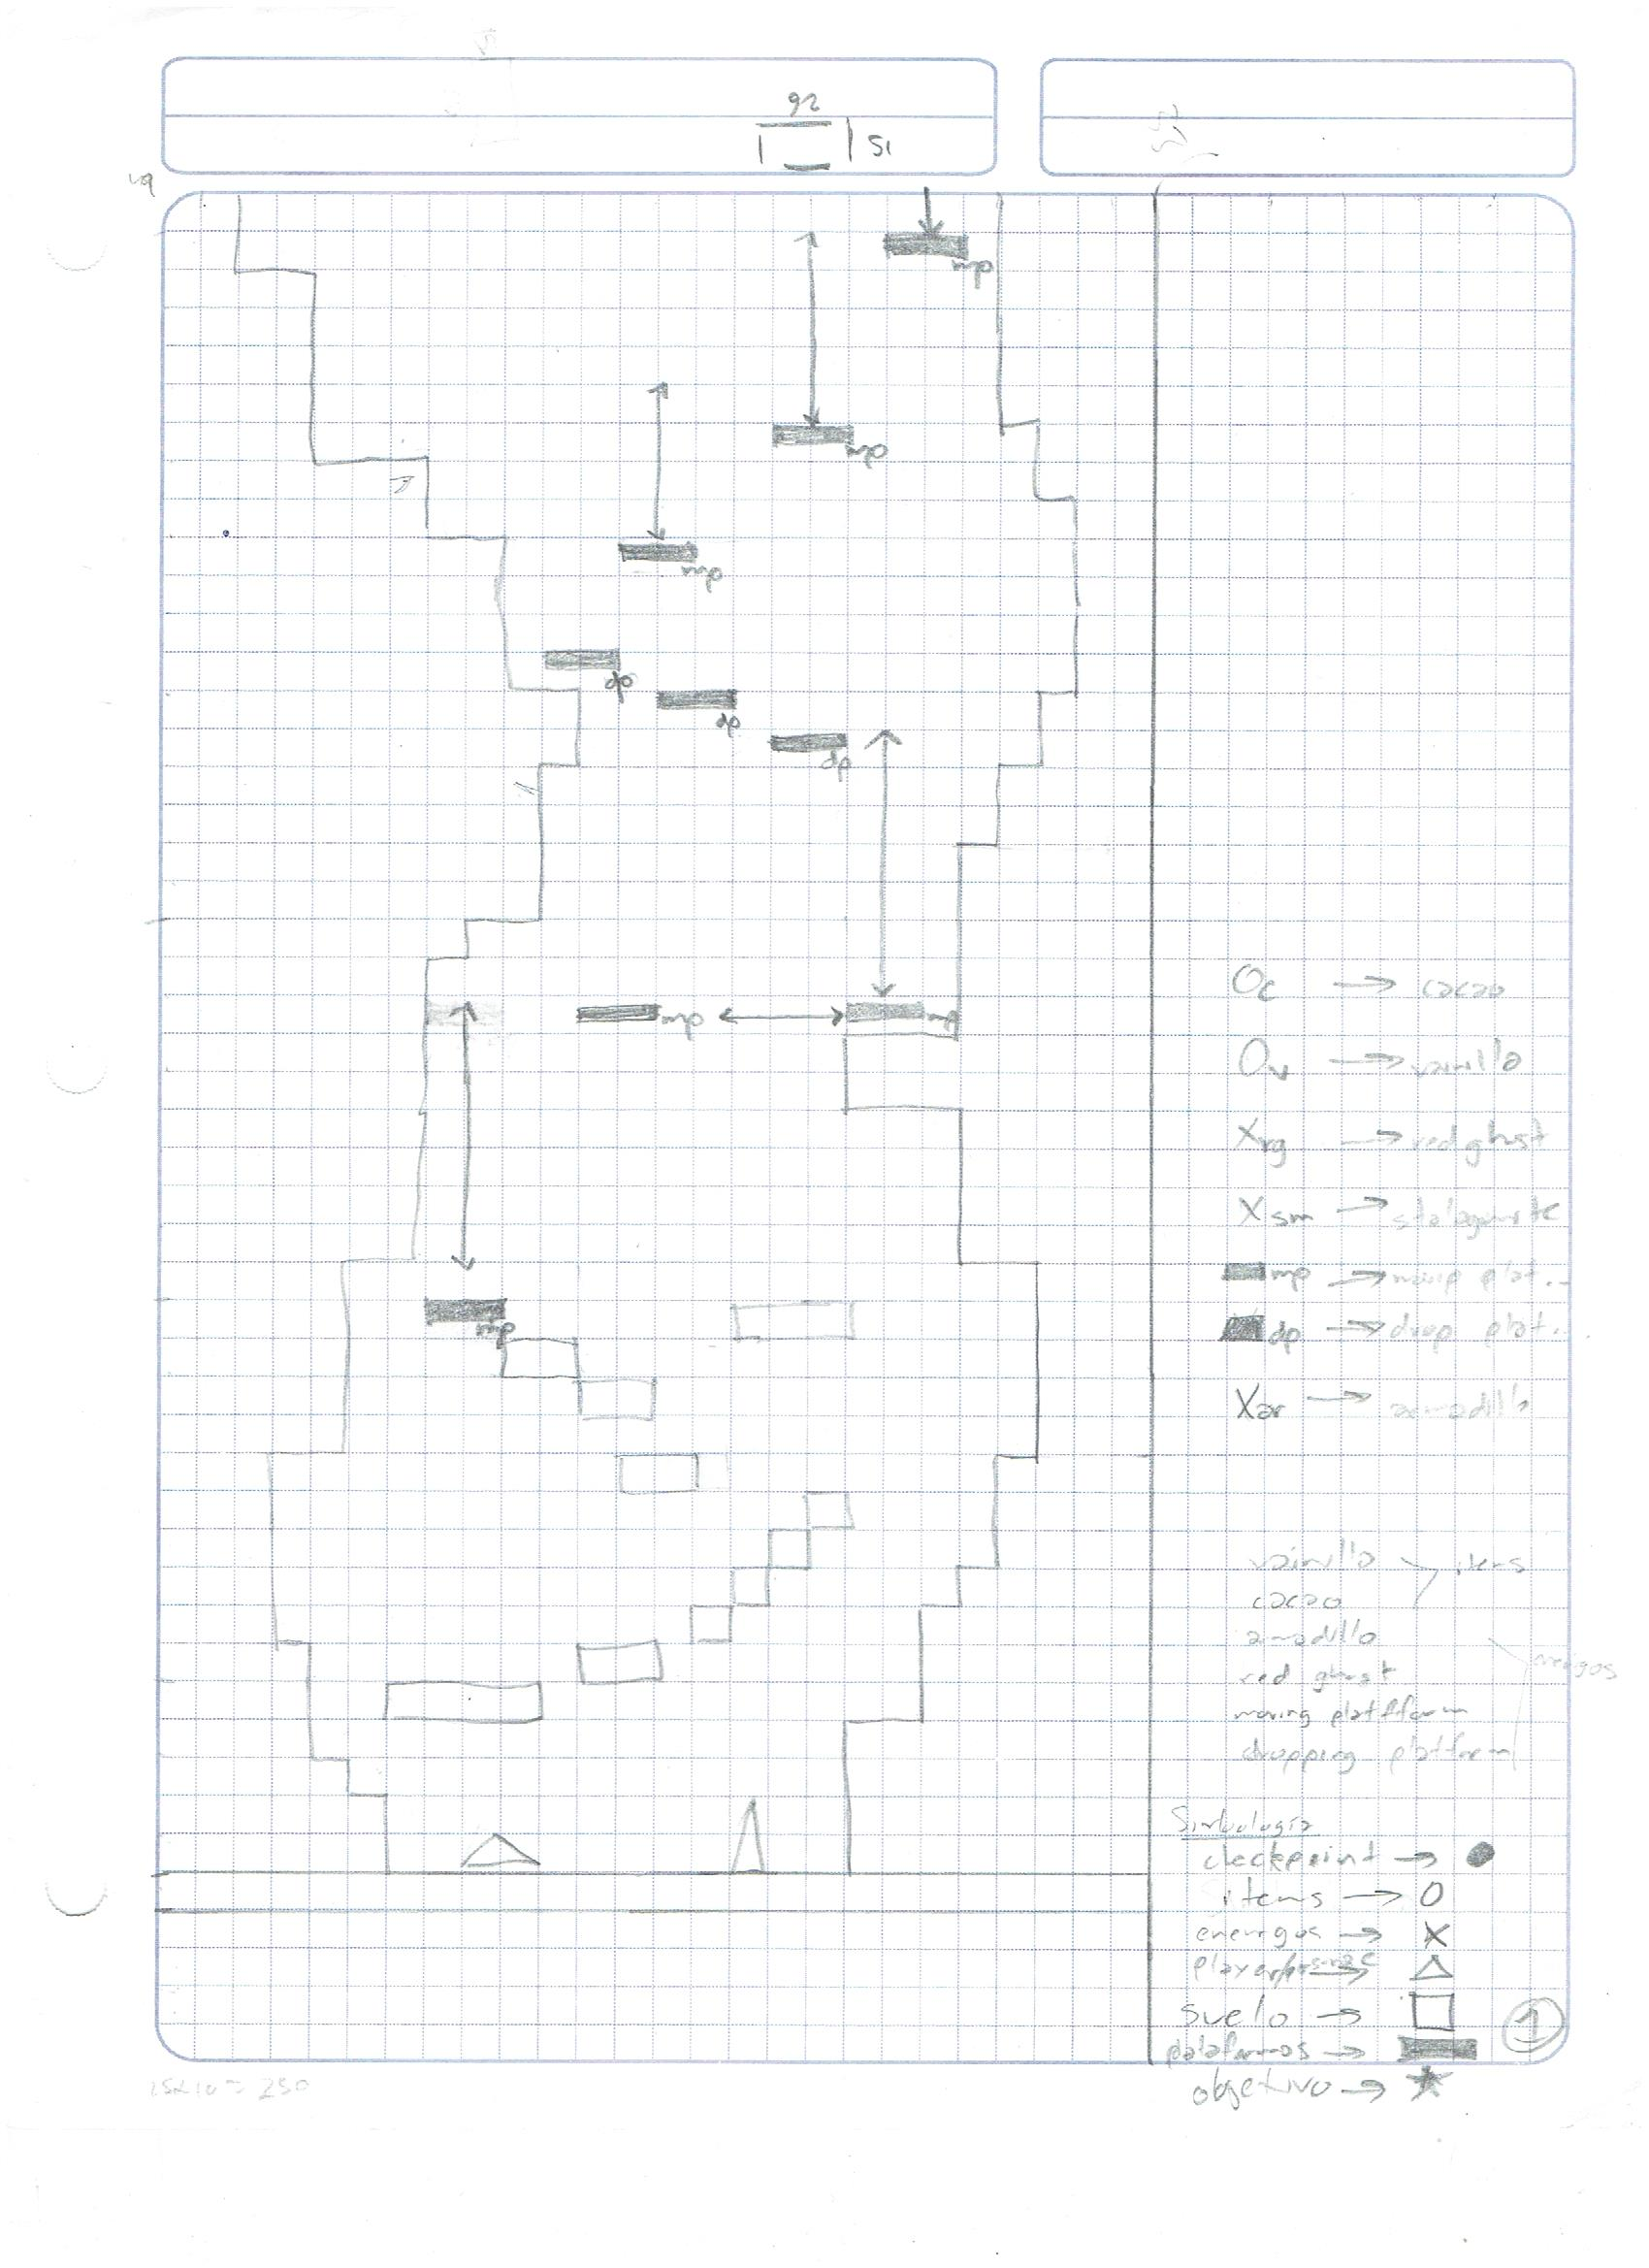
\includegraphics[width=5cm]{03TrabajoRealizado/DocProduccionR/imagenes/n3/01.jpg}}
	\subfigure[Segunda parte del nivel]{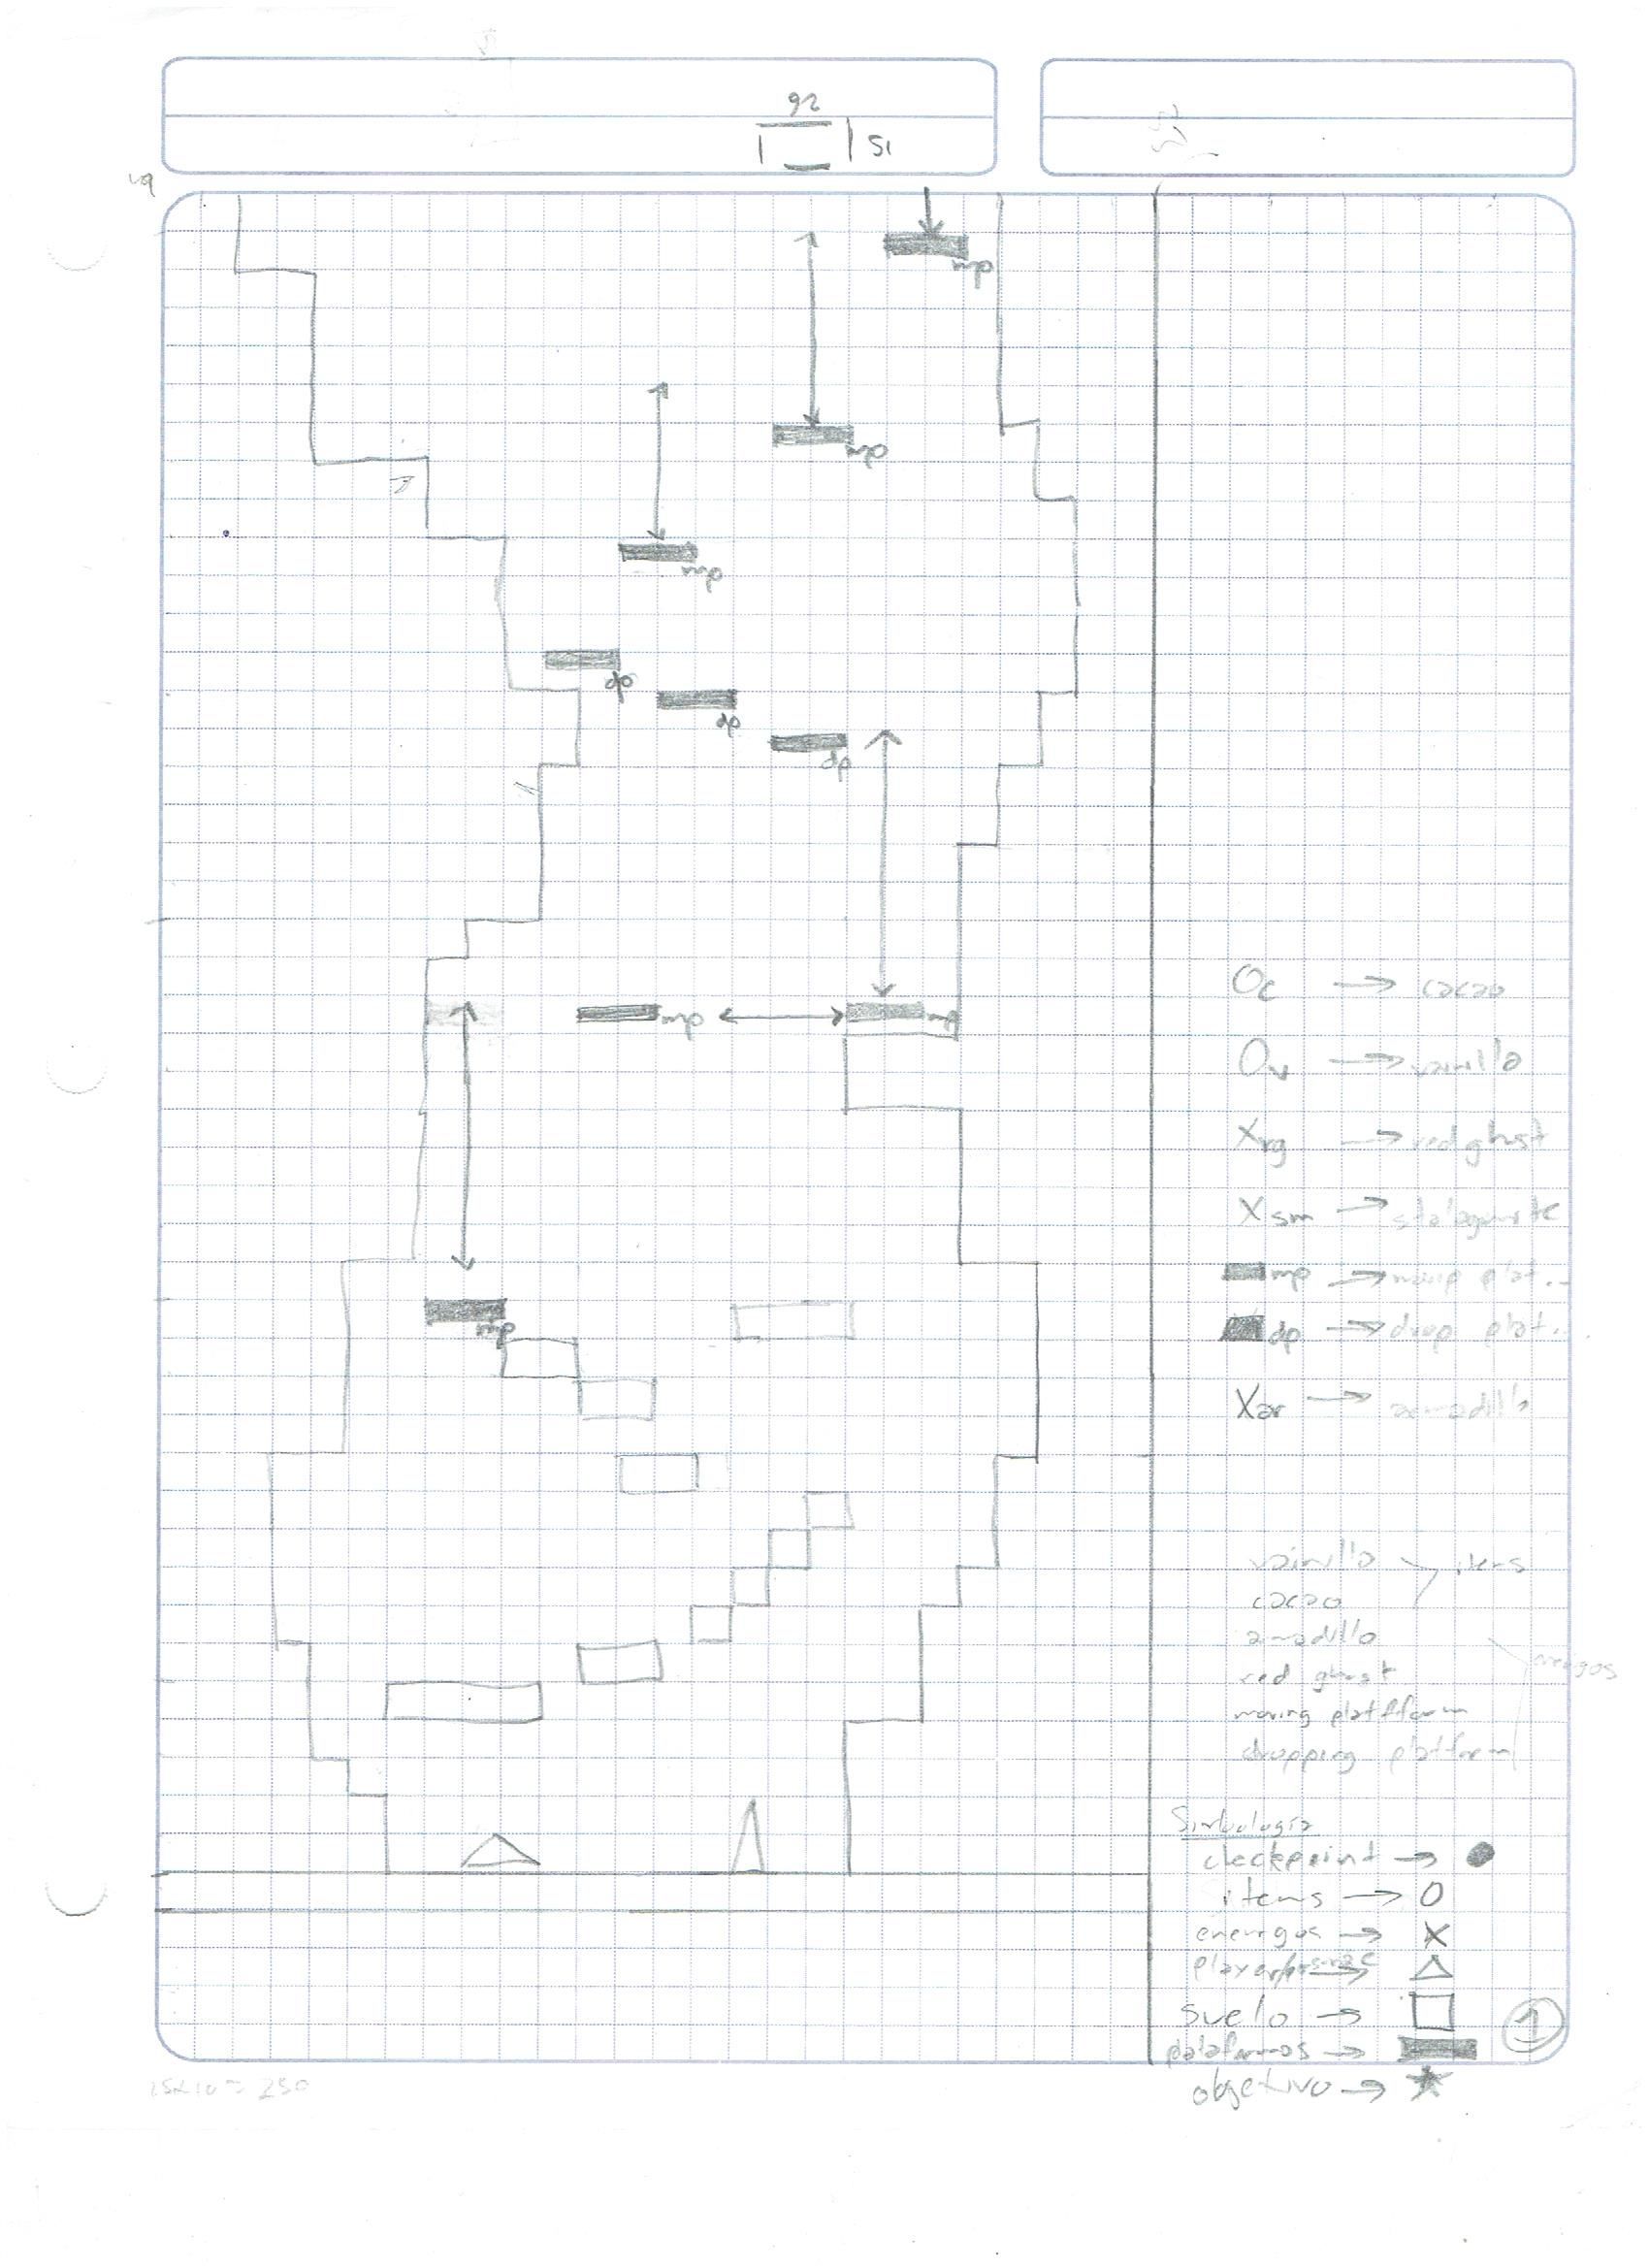
\includegraphics[width=5cm]{03TrabajoRealizado/DocProduccionR/imagenes/n3/02.jpg}}
	\subfigure[Tercera parte del nivel]{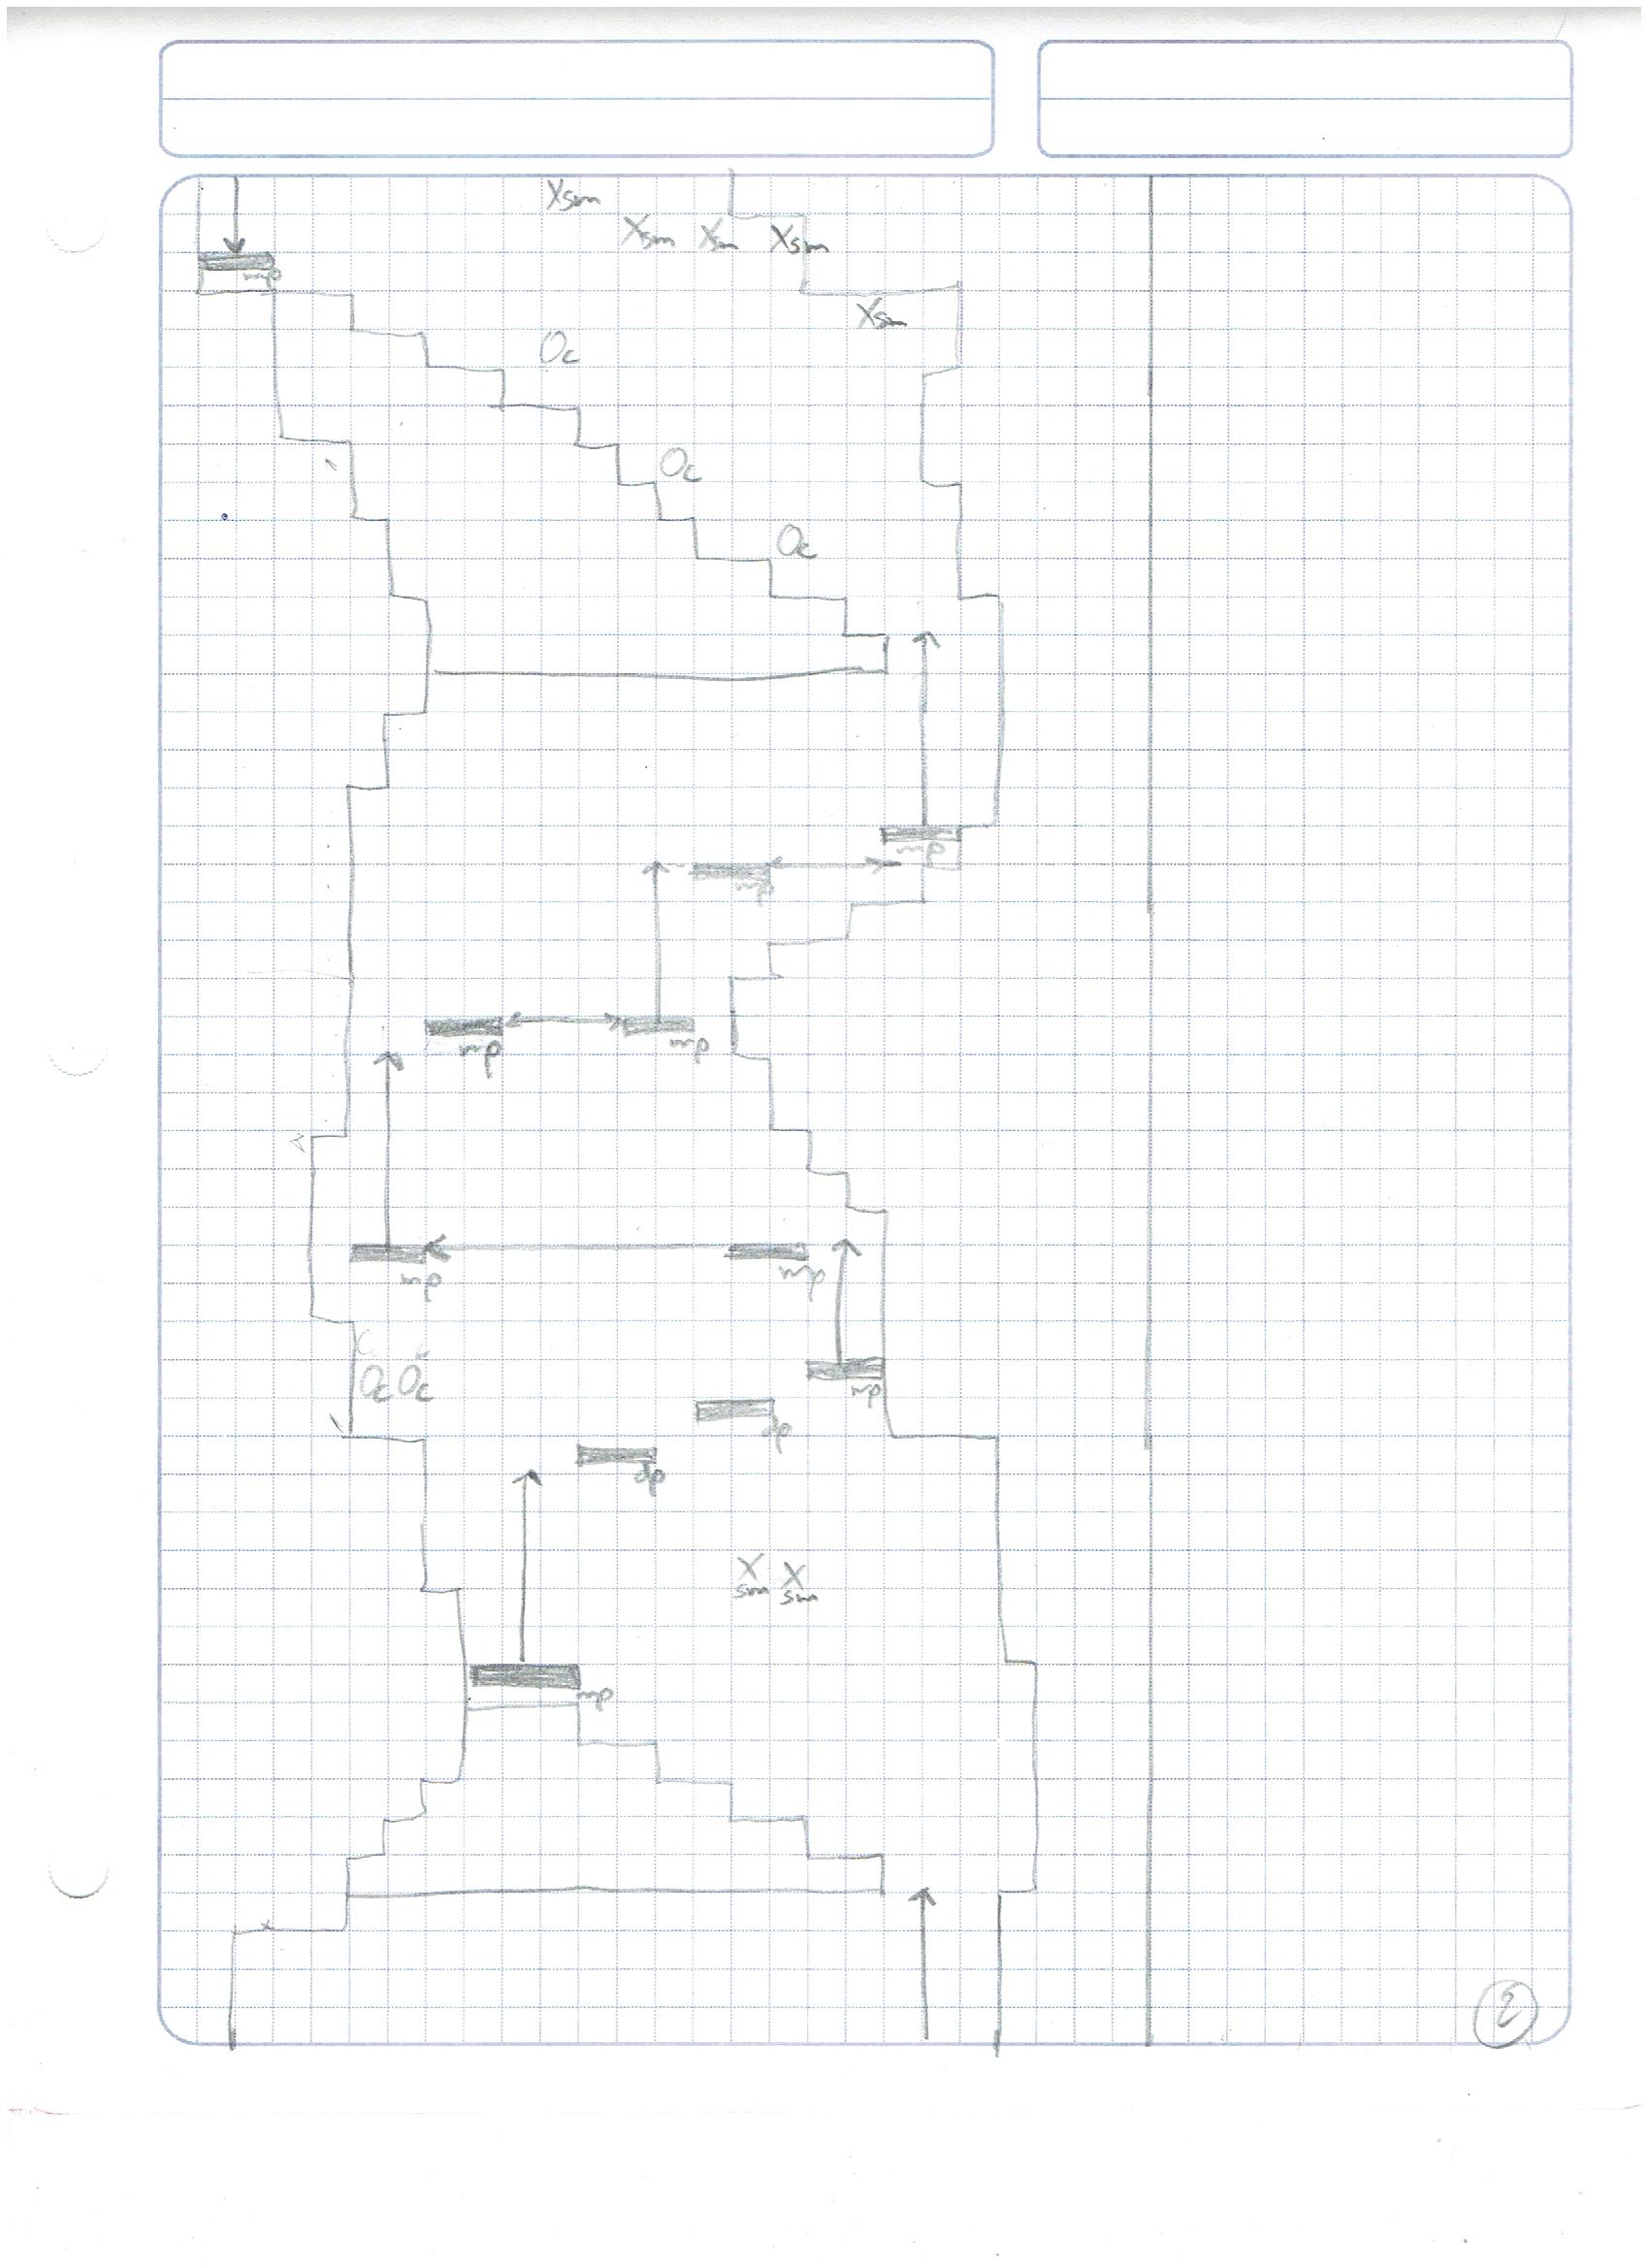
\includegraphics[width=5cm]{03TrabajoRealizado/DocProduccionR/imagenes/n3/03.jpeg}}
	\subfigure[Cuarta parte del nivel]{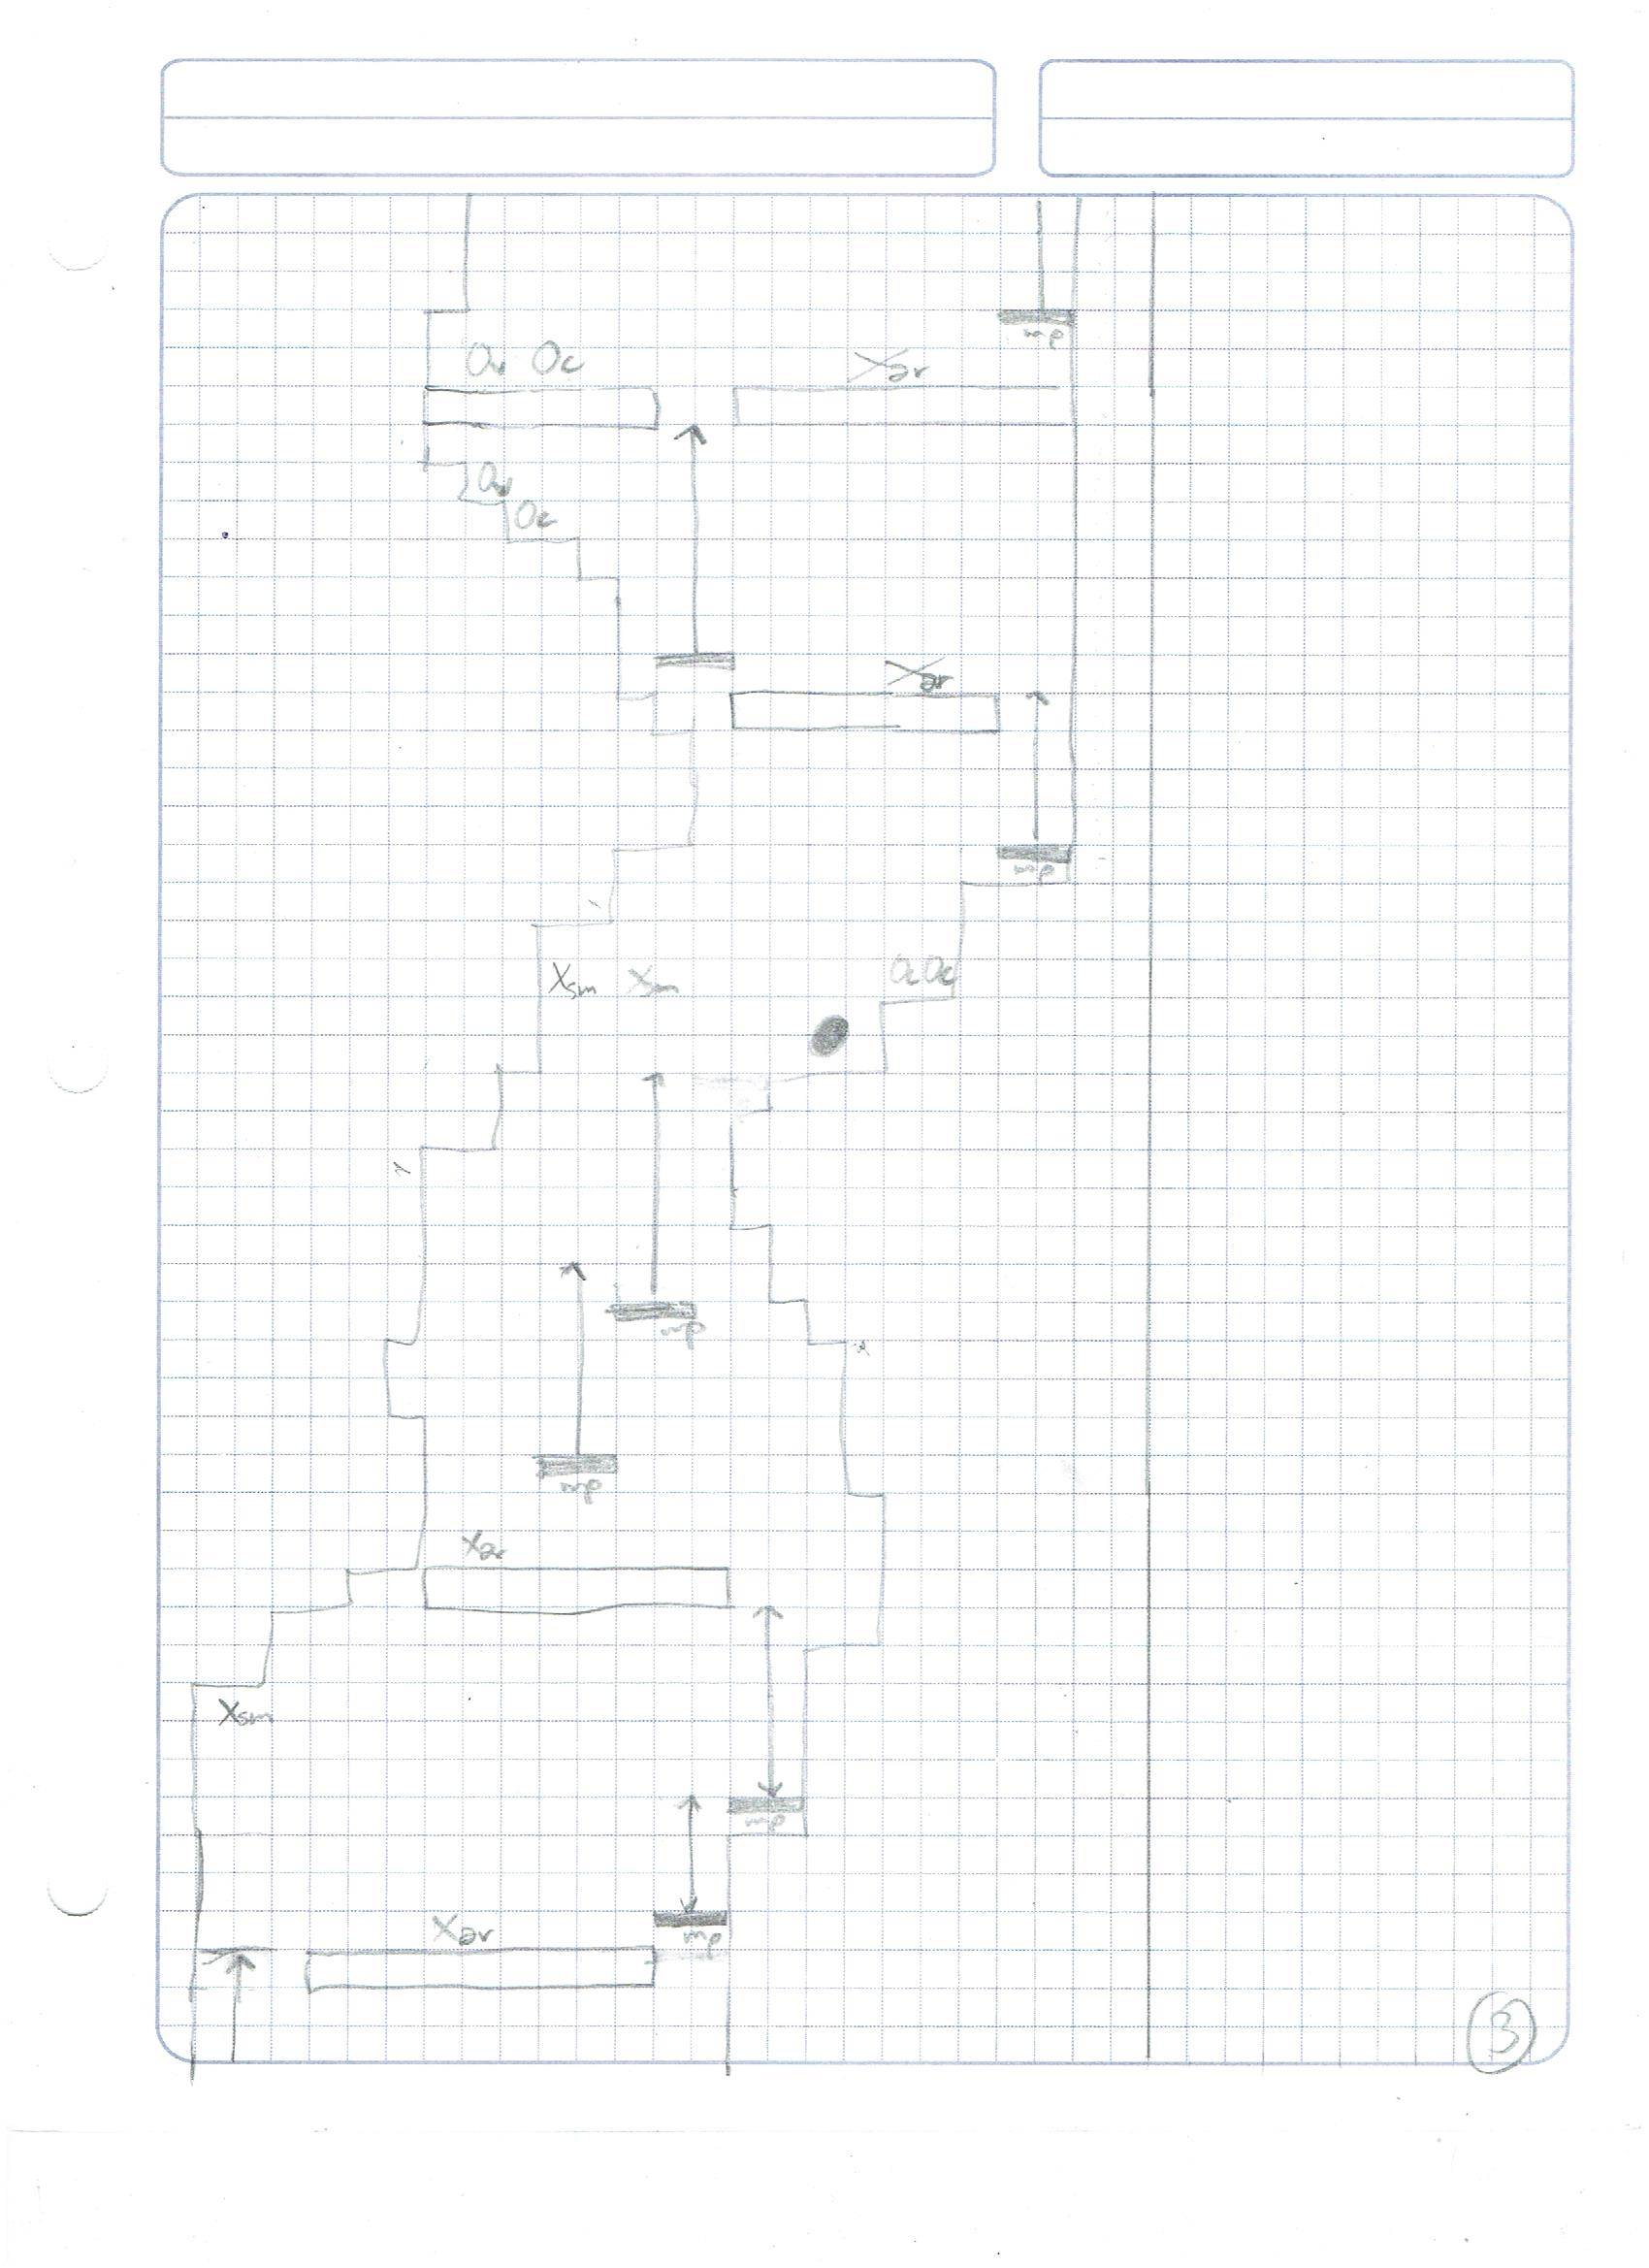
\includegraphics[width=5cm]{03TrabajoRealizado/DocProduccionR/imagenes/n3/04.jpg}}
	\caption{Maquetado de nivel tres} \label{fig:n01}
\end{figure}  

Después se lleva la tarea de tomar todos los componentes solo de manera visual y adecuar el tamaño necesario, tomando en cuenta las medidas de los componentes anteriores. Dichas imágenes se pueden ver en la \ref{fig:n02}.
\begin{figure}[htbp]
	\centering
	\subfigure[Imagen de cacao para recuperar vida]{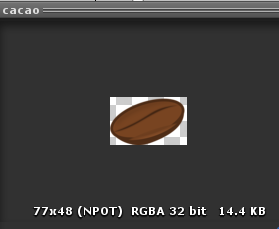
\includegraphics[width=5cm]{03TrabajoRealizado/DocProduccionR/imagenes/n3/n302.png}}
	\subfigure[Imagen de enemigo fantasma rojo]{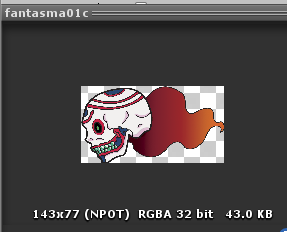
\includegraphics[width=5cm]{03TrabajoRealizado/DocProduccionR/imagenes/n3/n303.png}}
	\subfigure[Imagen de rugido de jefe enemigo]{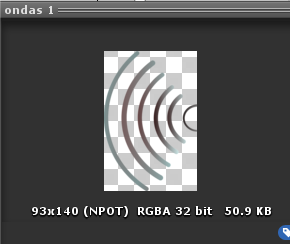
\includegraphics[width=5cm]{03TrabajoRealizado/DocProduccionR/imagenes/n3/n304.png}}
	\subfigure[Imagen de roca utilizada para daño]{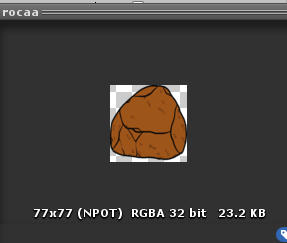
\includegraphics[width=5cm]{03TrabajoRealizado/DocProduccionR/imagenes/n3/n305.png}}
	\subfigure[Imagen de jefe enemigo jaguar Tepeyóllotl]{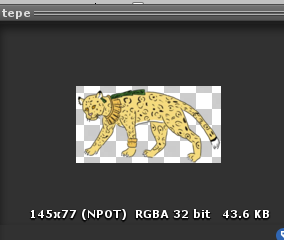
\includegraphics[width=5cm]{03TrabajoRealizado/DocProduccionR/imagenes/n3/n306.png}}
	\subfigure[Imagen de indicador de cambio de escena]{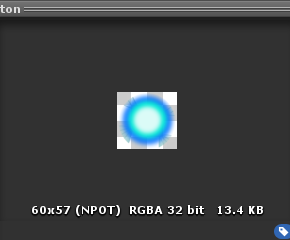
\includegraphics[width=5cm]{03TrabajoRealizado/DocProduccionR/imagenes/n3/n307.png}}
	\subfigure[Imagen de cara de jefe enemigo jaguar como indicador]{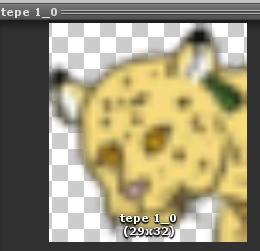
\includegraphics[width=5cm]{03TrabajoRealizado/DocProduccionR/imagenes/n3/n308.png}}
	\subfigure[Imagen de flor de vainilla para recuperar tonalli]{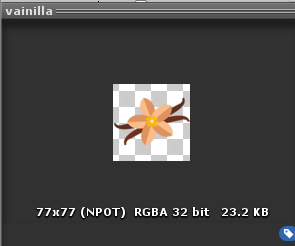
\includegraphics[width=5cm]{03TrabajoRealizado/DocProduccionR/imagenes/n3/n309.png}}
	\subfigure[Imagen de enemigo armadillo]{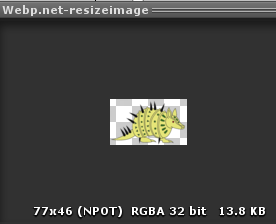
\includegraphics[width=5cm]{03TrabajoRealizado/DocProduccionR/imagenes/n3/n310.png}}
	\subfigure[Imagen de terreno rocoso]{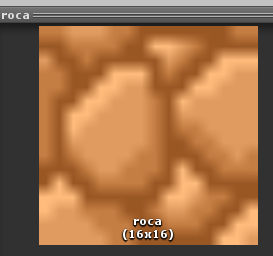
\includegraphics[width=5cm]{03TrabajoRealizado/DocProduccionR/imagenes/n3/n311.png}}
	\subfigure[Imagen de terreno con pasto]{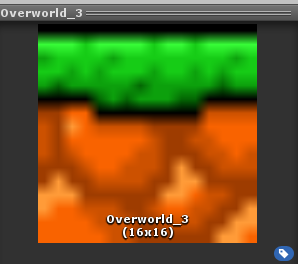
\includegraphics[width=5cm]{03TrabajoRealizado/DocProduccionR/imagenes/n3/n312.png}}
	\subfigure[Imagen de roca gigante]{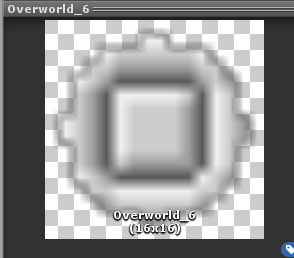
\includegraphics[width=5cm]{03TrabajoRealizado/DocProduccionR/imagenes/n3/n313.png}}
	\caption{Imágenes utilizadas para el nivel} \label{fig:n02}
\end{figure}

Después de reunir los componentes se da a la tarea de dar las acciones que realizarían descritas dentro de la figura \ref{fig:n03}. Se omite en esta parte los fantasmas enemigos que ya han sido realizados en niveles anteriores.
\begin{figure}[htbp]
	\centering
	\subfigure[Establecer que los picos tengan detección por debajo de ellos y despues caer para realizar daño.]{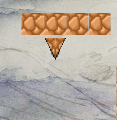
\includegraphics[width=5cm]{03TrabajoRealizado/DocProduccionR/imagenes/n3/lo0.png}}
	\subfigure[Establecer que la roca gigante detecte en una zona establecida el pase del jugador y después caiga rodando para estorbar el paso.]{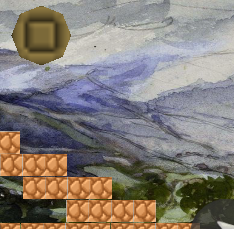
\includegraphics[width=5cm]{03TrabajoRealizado/DocProduccionR/imagenes/n3/lo1.png}}
	\subfigure[Ejemplo muestra de las plataformas que se mueven en dirección horizontal, la del lado izquierdo y vertical, la del lado derecho.]{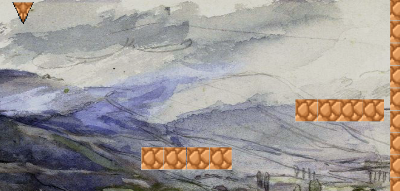
\includegraphics[width=5cm]{03TrabajoRealizado/DocProduccionR/imagenes/n3/lo2.png}}
	\subfigure[Piso que al tener contacto con el jugador este toma otra posición más abajo.]{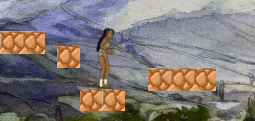
\includegraphics[width=5cm]{03TrabajoRealizado/DocProduccionR/imagenes/n3/lo3.png}}
	\subfigure[Ejemplo de como una vez que el jugador se quita de la posición sobre el piso, este vuelve a su lugar.]{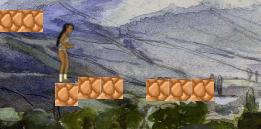
\includegraphics[width=5cm]{03TrabajoRealizado/DocProduccionR/imagenes/n3/lo4.png}}
	\caption{Muestra de comportamiento de objetos} \label{fig:n03}
\end{figure}

Ya que se tiene los objetos con los comportamientos deseados se procede a ubicarlos según correspondan como se ve en la \ref{fig:n04}.
\begin{figure}
	\centering
	\caption{Maquetado llevado al motor de juego Unity.}
	\label{fig:n04}
	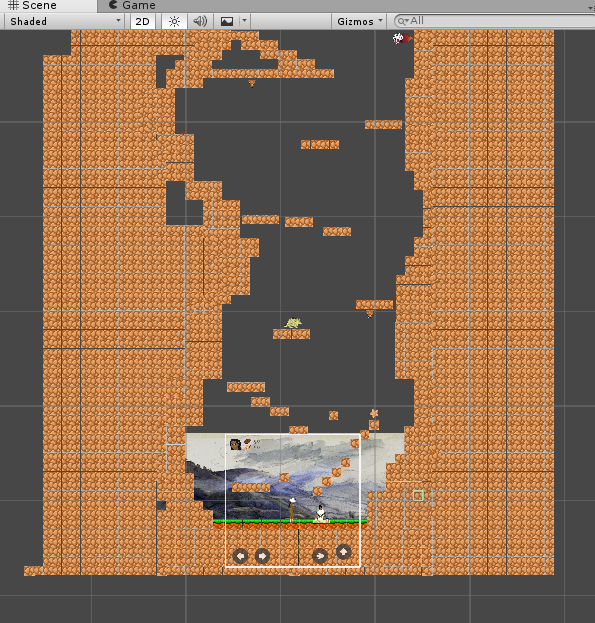
\includegraphics[width=0.5\textwidth]{03TrabajoRealizado/DocProduccionR/imagenes/n3/n301.png}
\end{figure}

Por último se establece las acciones que realiza el jefe enemigo Tepeyóllotl descritas en la siguiente figura \ref{fig:n05}.
\begin{figure}[htbp]
	\centering
	\subfigure[El enemigo se lanza en dirección al jugador con otro color.]{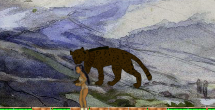
\includegraphics[width=5cm]{03TrabajoRealizado/DocProduccionR/imagenes/n3/n314.png}}
	\subfigure[El enemigo aparece rocas que van cayendo desde la parte superior.]{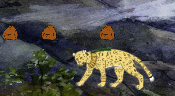
\includegraphics[width=5cm]{03TrabajoRealizado/DocProduccionR/imagenes/n3/n315.png}}
	\subfigure[El enemigo realiza un rugido.]{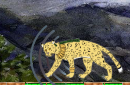
\includegraphics[width=5cm]{03TrabajoRealizado/DocProduccionR/imagenes/n3/n316.png}}
	\subfigure[El enemigo realiza un azote contra el piso apareciendo rocas a sus lados.]{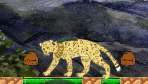
\includegraphics[width=5cm]{03TrabajoRealizado/DocProduccionR/imagenes/n3/n317.png}}
	\caption{Muestra de acciones de el jefe enemigo jaguar} \label{fig:n05}
\end{figure}

\section{Cuarto \textit{sprint} de producción}
Una vez definidas las nuevas estrategias de trabajo y que se atendieron 
las observaciones de los sinodales se procedió a realizar la maquetación de los 
niveles pares restantes y los \textit{sprites} faltantes. Al termino de este 
\textit{sprint} se obtienen más de 100 \textit{sprites} y las maquetas de los 
niveles pares.

\subsection{Creación de las maquetas de los niveles pares restantes}
Para la generación de las maquetas se sigue usando la plantilla creada durante 
la creación del primer demo del juego (ver figura \ref{fig:MaquetaPlantilla}). 
Para la creación de la maqueta también se crea un documento con todos los 
componentes de un nivel como son los enemigos, los ítems, los puntos de guardado, 
las plataformas y los obstáculos. Este documento se imprime y los objetos se 
recortan para ser pegados como estampas en las plantillas de diseño de las 
maquetas. En promedio la maqueta de cada nivel no excede de las 15 plantillas, 
sin embargo hay algunas que exceden este numero como la maqueta del cuarto nivel, 
la cual por su naturaleza de laberinto termino por ser más extensa que el 
resto. Por su parte los niveles correspondientes a los jefes de los niveles no 
sobrepasan de las tres plantillas, siendo la maqueta del jefe del sexto nivel 
la más pequeña de todas. 

%%
\begin{figure}[h]
	\centering
	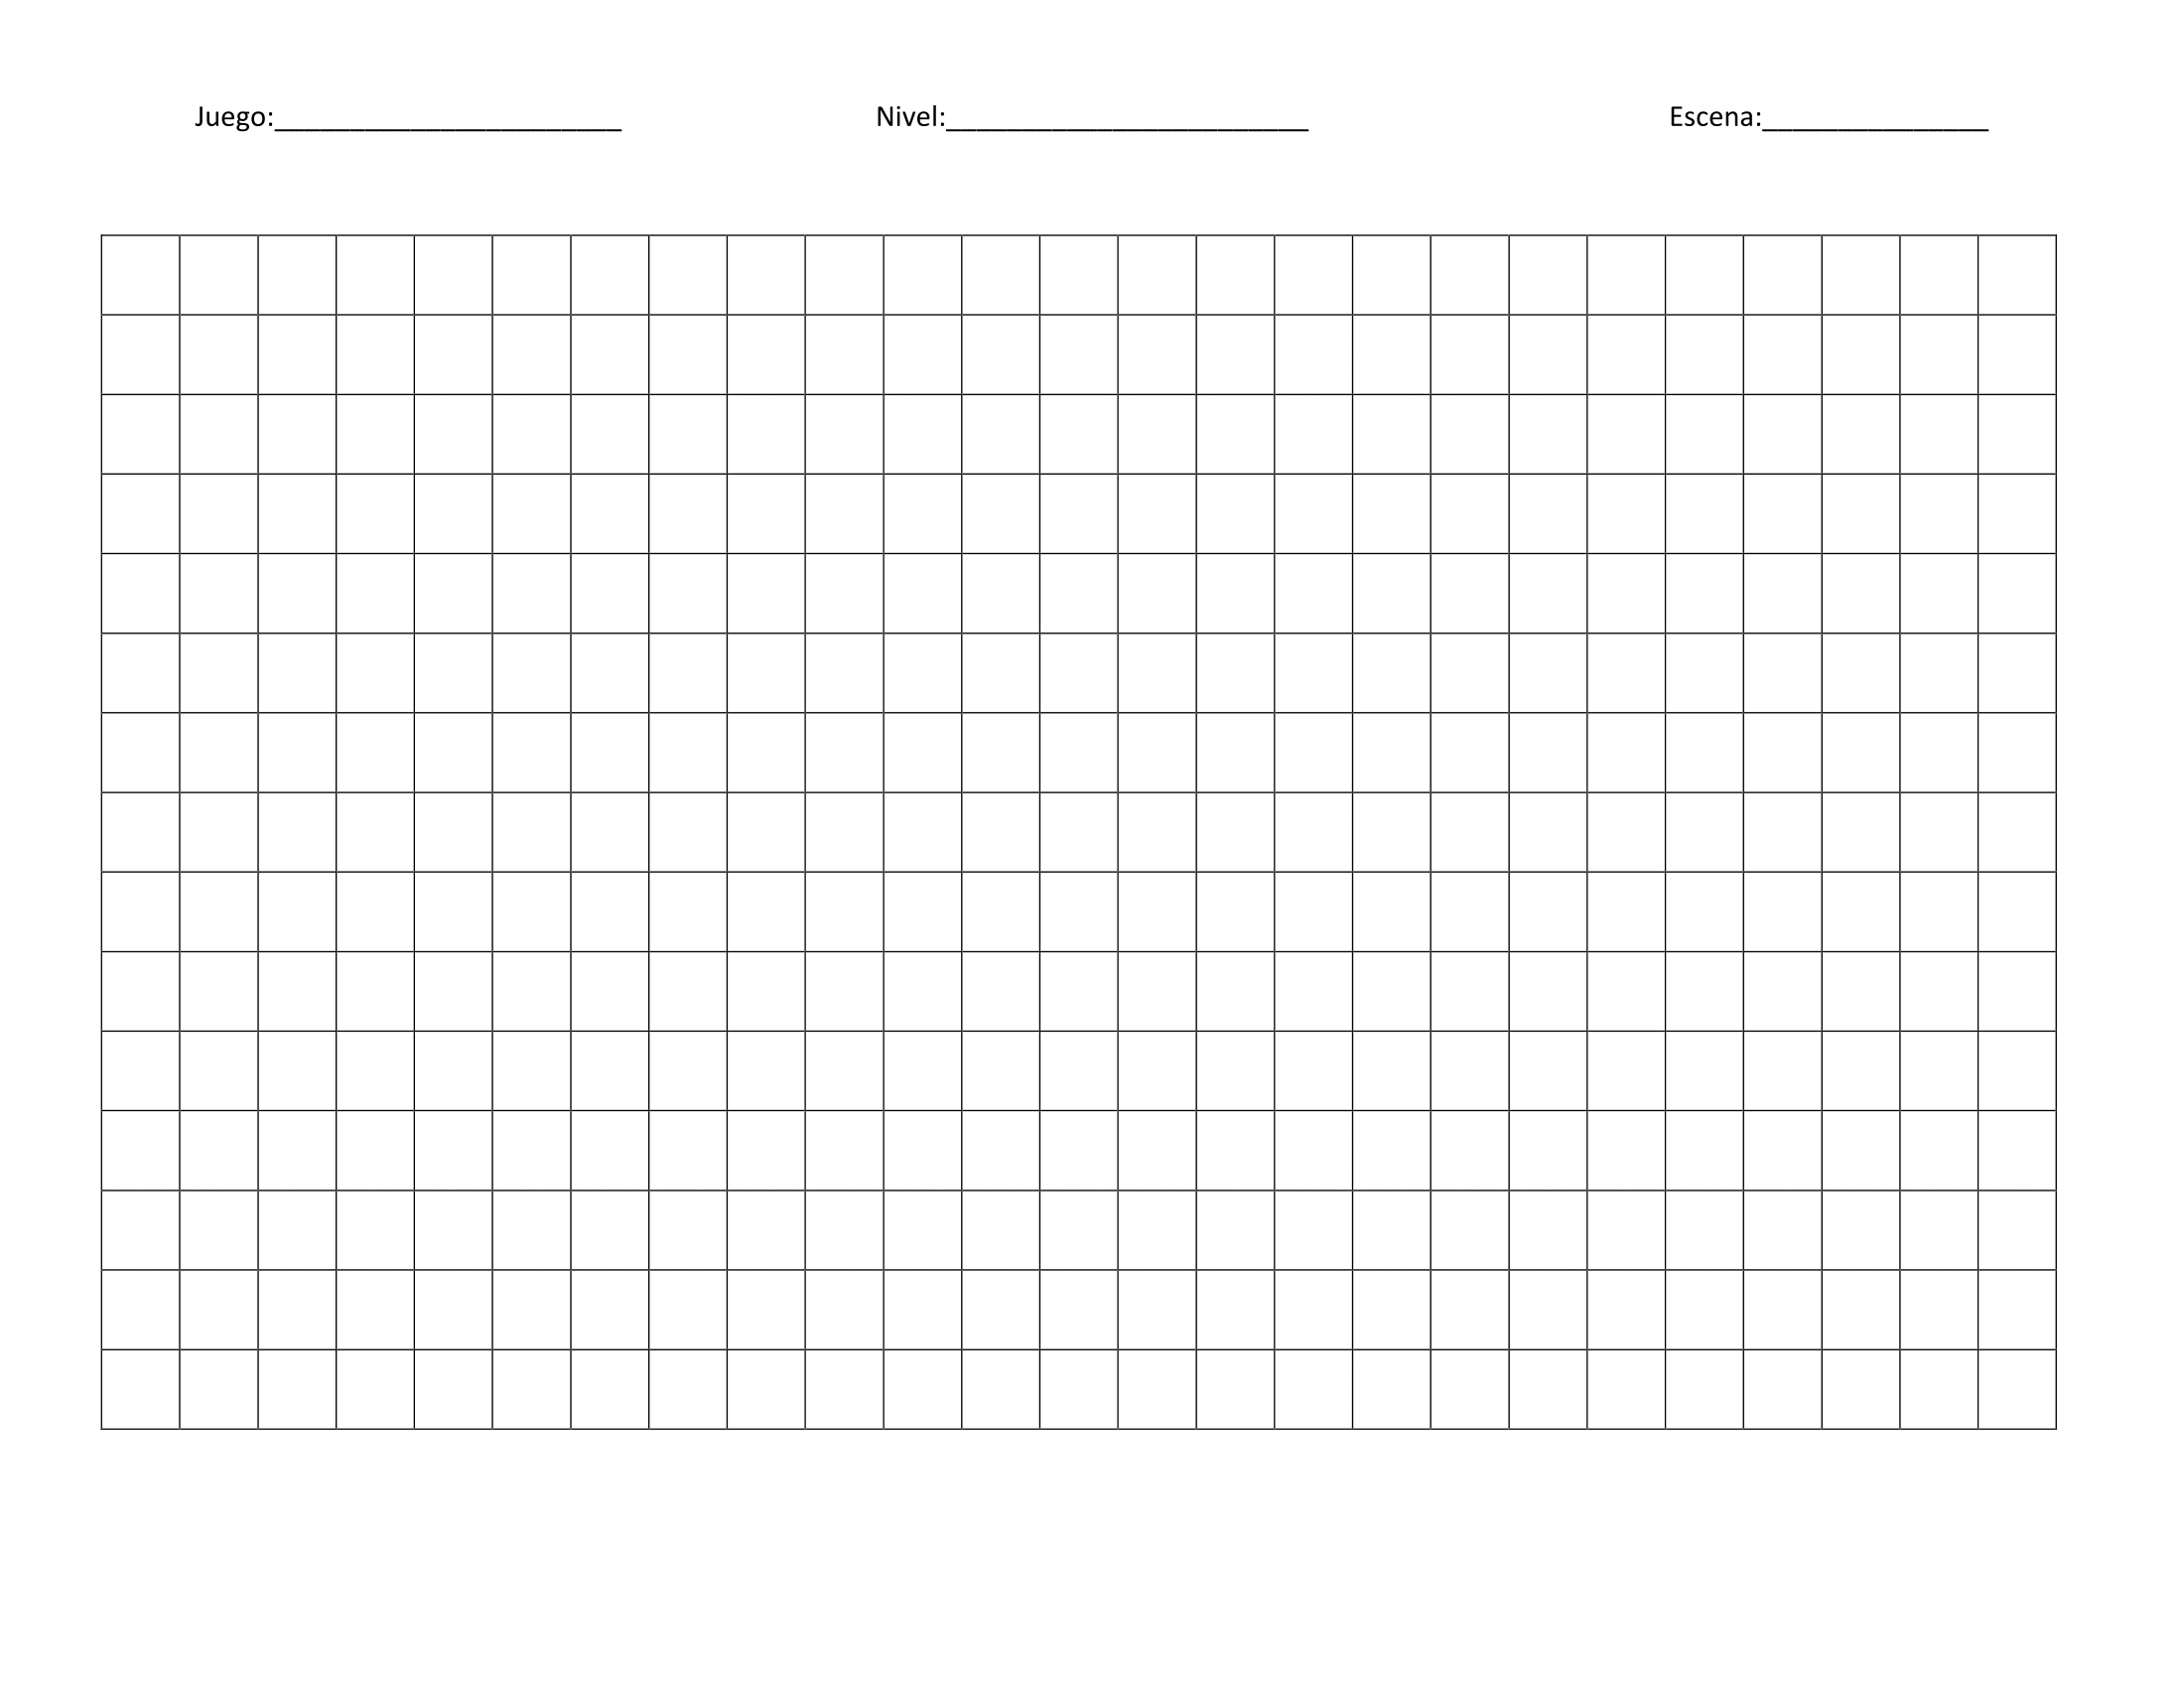
\includegraphics[width=0.6\textwidth]{03TrabajoRealizado/imagenes/maqueta-1.png}
 	\caption{Plantilla para la crecaión de niveles.}
	\label{fig:MaquetaPlantilla}		
\end{figure}

\subsection{Creación de los \textit{sprites} faltantes}
Lo siguiente a realizarse durante el cuarto \textit{sprint} fueron los \textit{sprites}, 
durante las modificaciones que se definieron en Trabajo Terminal 1 fue la 
utilización de un \textit{software} de animación en dos dimensiones para generar 
los \textit{sprites} restantes; sin embargo, el cambio de \textit{software} para 
generar los sprites fue descartado, esto debido a que se adquirió una nueva 
tableta digitalizadora que agilizó la creación de \textit{sprites}. Para Trabajo 
Terminal 2 se dibujaron y digitalizaron más de 100 \textit{sprites}. Para mejorar 
la experiencia visual del jugador se animaron \textit{sprites} que en los primeros 
demos eran estáticos como es el caso de los fantasmas del segundo nivel de la 
sección de plataformas (ver figura \ref{fig:FantasmaAnimacion}). 

%%
\begin{figure}[h]
	\centering
	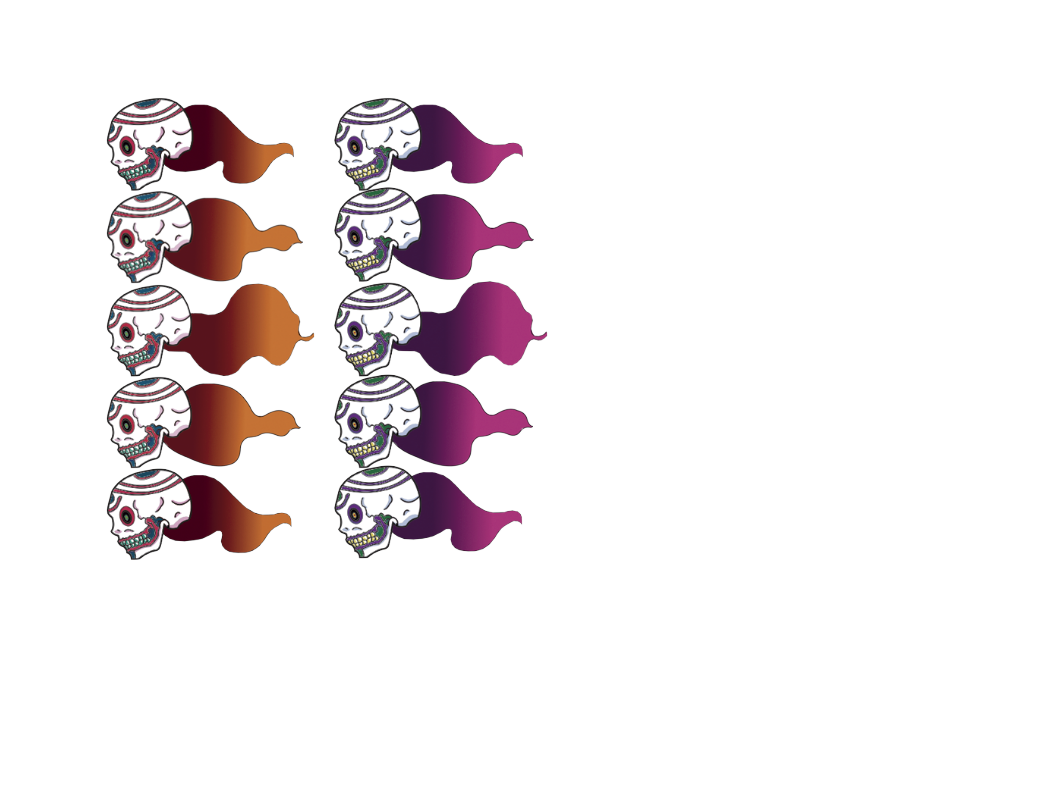
\includegraphics[width=0.6\textwidth]{03TrabajoRealizado/imagenes/fantasmas.png}
 	\caption{Bloques de animación para el enemigo de tipo fantasma.}
	\label{fig:FantasmaAnimacion}		
\end{figure}

Otros cambios en cuanto el aspecto visual del juego fue la integración de nuevos 
\textit{sprites} para el personaje jugable, los nuevos sprites incluyen la 
caracola que \textit{Malinalli} (ver figura \ref{fig:MalinalliCaracola}) emplea 
para atacar y que se obtiene al final del primer nivel de la sección de selva, 
estos \textit{sprites} para \textit{Malinalli} son utilizados únicamente en los 
niveles posteriores al primer nivel para darle sentido a la narrativa; para el 
segundo nivel se hizo algo parecido, los \textit{sprites} del personaje jugable 
fueron sustituidos por \textit{Malinalli} montando un ajolote (ver figura 
\ref{fig:MalinalliAjolote}), este cambio se hizo para que lo que el jugador vea 
dentro del nivel sea coherente con la narrativa propuesta y se mejore la inmersión del juego. 

\begin{figure}[h]
	\centering
	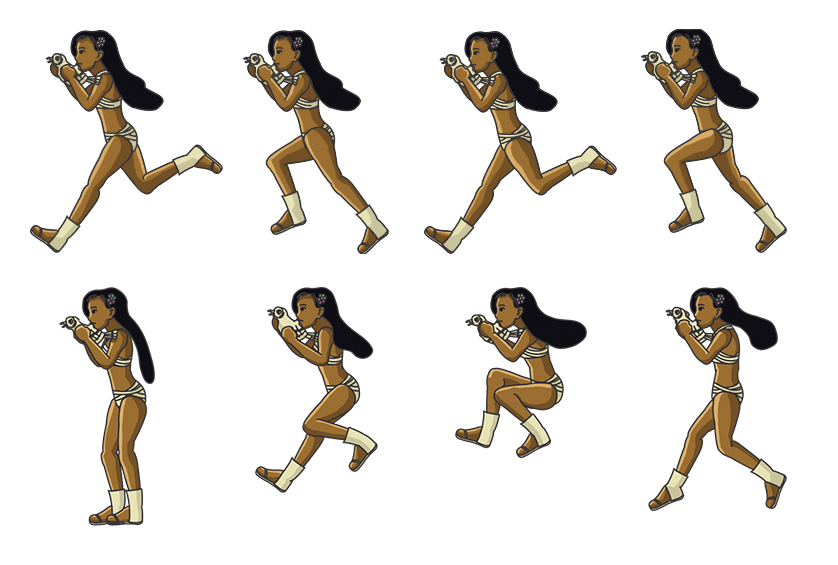
\includegraphics[width=0.4\textwidth]{03TrabajoRealizado/imagenes/MalinalliArma.png}
 	\caption{Bloques de animación para \textit{Malinalli} posterior a que ella obtiene la caracola.}
	\label{fig:MalinalliCaracola}		
\end{figure}

\begin{figure}[h]
	\centering
	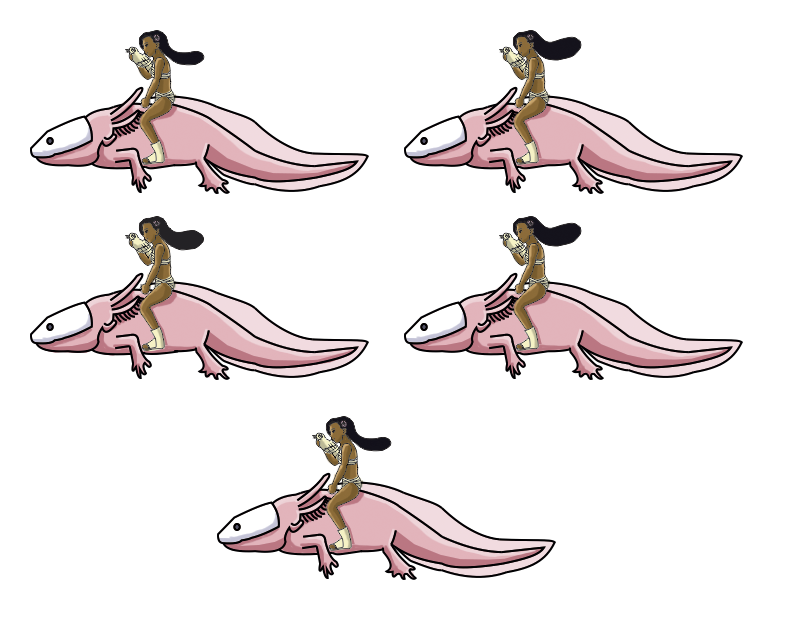
\includegraphics[width=0.5\textwidth]{03TrabajoRealizado/imagenes/MalinaliAjolote.png}
 	\caption{Bloques de animación para \textit{Malinalli} montando al ajolote del segundo nivel del juego.}
	\label{fig:MalinalliAjolote}		
\end{figure}

En lo que se refiere a los Jefes de cada nivel, no solo se crearon sus 
respectivos \textit{sprites}, también fue necesario la creación de los 
\textit{sprites} referentes a sus ataques, para el caso particular de 
\textit{Mictlantecuhtli} se dibujaron 30 \textit{sprites} tanto para la animación 
del personaje como para la animación de sus respectivos ataque (ver figura 
\ref{fig:Mictlantecutli}). Para el diseño de la interfaz gráfica de usuario
(\textit{GUI} por sus siglas en íngles) se emplearon \textit{sprites} de las 
paginas \textit{Kenney.nl} y \textit{Game Art 2D}. Es importante aclarar que la 
creación de \textit{sprites} pudo haber sido sustituida utilizando paquetes de 
\textit{sprites} que existen en la red y que son de licencia libre; sin embargo, 
con la creación de \textit{sprites} propios para el juego se consigue crearle una 
identidad visual propia al juego, esto permite que el jugador se identifique con 
mayor facilidad con el personaje y tenga una mejor asociación con el mundo y la 
historia que se le presenta dentro del juego [cita]. Si se desea ver a profundidad 
los {sprites} que se crearon se puede consultar el anexo \ref{Anexo:Personajes}. 


\begin{figure}[h]
	\centering
	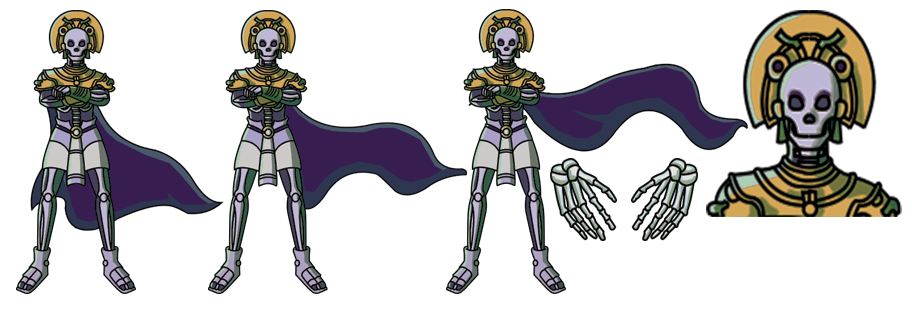
\includegraphics[width=0.6\textwidth]{03TrabajoRealizado/imagenes/Mictlantecuhtli.png}
 	\caption{Bloques de animación para \textit{Mictlantecuhtli}, jefe final del juego.}
	\label{fig:Mictlantecutli}		
\end{figure}

\subsection{Cierre del sprint}
Al terminar este \textit{sprint} se obtienen todas las maquetas de los niveles 
pares y los \textit{sprites} a utilizar de los mismos. Este \textit{sprint} se 
considera completado ya que se generaron todos los elementos que se tenían 
planeado. Como ultimo paso para este \textit{sprint}, se realiza el empaquetado 
de todos los \textit{sprites} creados durante el \textit{sprint}. 
\subsection{Detalles del proyecto}
Aquí se mostrará del proyecto el título, estudio, género, plataforma, fecha de inicio, fecha de término, lo planeado, en desarrollo, sin planear y terminado.
\\
\subsubsection{Título}
Yolotl

\subsubsection{Estudio}
ESCOM - IPN

\subsubsection{Plataforma}
Dispositivos móviles android

\subsubsection{Fecha de inicio}
26 febrero 2018
\subsubsection{Fecha de término}
1 Abril 2018
\subsubsection{Planeado}
El 48\%
\subsubsection{Desarrollo}
El 42\%
\subsubsection{Planear}
El 20\%
\subsubsection{Terminado}
El 32\%



\subsection{Sprint plan}
\subsubsection{SprintID}
05
\subsubsection{Inicio}
12 Marzo 2018
\subsubsection{Días}
7
\subsubsection{Fin}
18 Marzo 2018
\subsubsection{Meta}
Nivel 5
\subsubsection{Porcentaje}
El 16\% 


\subsection{Project chart}



\subsection{Feature log}

\subsubsection{FeatureID}
05
\subsubsection{Nombre}
N5
\subsubsection{Estado}
Planeado
\subsubsection{Días}
7
\subsubsection{SprintID}
05
\subsubsection{Comentarios}
-


\subsection{Sprint backlog}
\subsubsection{Sprint # backlog}
05
\subsubsection{Días}
7
\subsubsection{Tareas}
14
\subsubsection{Tendencia}
0
\subsubsection{Esfuerzo restante}
56
\subsubsection{Tendencia actual}
-
\subsubsection{Progreso ideal}
14
\subsubsection{Tareas restantes}
14
\subsubsection{Nombre de la tarea}
n5
\subsubsection{FeatureID}
05
\subsubsection{Miembro}
Rocío
\subsubsection{Rol}
Desarrollo
\subsubsection{Estado}
Planeado
\subsubsection{Esfuerzo}
14
\subsubsection{Números}



\subsection{Task chart - sprint "ggrafica"}



\subsection{Burn-down chart "grafica"}


\subsection{Task Slips}


\subsubsection{FeatureID}5
\subsubsection{Nombre}Maqueta
\subsubsection{Tarea}Realizar maqueta del nivel completo
\subsubsection{Miembro}Rocío
\subsubsection{Esfuerzo estimado}1
\subsubsection{Terminado}si
\subsubsection{Restante}0


\subsubsection{FeatureID} 5
\subsubsection{Nombre} Enemigos
\subsubsection{Tarea} Realizar el comportamiento de los enemigos o cualquier otra acción necesaria dentro del nivel
\subsubsection{Miembro} Rocio
\subsubsection{Esfuerzo estimado} 5
\subsubsection{Terminado} sí
\subsubsection{Restante} 0


\subsubsection{FeatureID} 5
\subsubsection{Nombre} Arte 1
\subsubsection{Tarea} Crear vista de los personajes
\subsubsection{Miembro} Rocío
\subsubsection{Esfuerzo estimado} 2
\subsubsection{Terminado} sí
\subsubsection{Restante} 0



\subsubsection{FeatureID} 5
\subsubsection{Nombre} Arte 2
\subsubsection{Tarea} Crear el diseño de los obstáculos
\subsubsection{Miembro} Rocío
\subsubsection{Esfuerzo estimado} 2
\subsubsection{Terminado} sí
\subsubsection{Restante} 0


\subsubsection{FeatureID} 5
\subsubsection{Nombre} Arte 3
\subsubsection{Tarea} Crear el diseño de los items
\subsubsection{Miembro} Rocio
\subsubsection{Esfuerzo estimado} 2
\subsubsection{Terminado} sí
\subsubsection{Restante} 0

\subsubsection{FeatureID} 5
\subsubsection{Nombre} Boss 1
\subsubsection{Tarea} Diseñar la máquina de estados del enemigo principal del nivel
\subsubsection{Miembro} Rocio
\subsubsection{Esfuerzo estimado} 2
\subsubsection{Terminado} sí
\subsubsection{Restante} 0

\subsubsection{FeatureID} 5
\subsubsection{Nombre} Boss 2
\subsubsection{Tarea} Crear la máquina de estados del enemigo principal del nivel
\subsubsection{Miembro} Rocio
\subsubsection{Esfuerzo estimado} 2
\subsubsection{Terminado} sí
\subsubsection{Restante} 0

\section{Sexto \textit{sprint} de producción}
En este \textit{sprint} se tiene como objetivo la implementación de todos los
actores del juego tanto a nivel de código como en la creación de los
\textit{GameObjects} para generar su posterior \textit{Assets}. En esta sección
no se hablan de aquellos actores que se hayan implementado desde Trabajo terminal
1 a no ser que su funcionalidad se haya rediseñado.

\subsection{Implementando los enemigos normales del juego}
Las primeras clases actoras en ser programadas fueron las correspondientes a los
enemigos normales, estas clases se programaron a la par que la clase \textit{Player}.
Si bien la clase \textit{Player} ya estaba programada desde los primeros prototipos,
esta clase no contaba con toda su funcionalidad implementada y la funcionalidad
faltante tuvo que ser implementada a la par que otras clases para verificar el
correcto funcionamiento en la interacción de clases como la de los enemigos y los
\textit{ítems}.
\\
\par
Al igual que con la clase \textit{Player},  existían enemigos desde los primeros prototipos; no obstante,
su funcionalidad tuvo que volver a ser implementada a fin de ofrecer un desempeño que
optimice recursos y agregue nuevas funcionalidades. A continuación, se listan los
cambios que presentan los enemigos de séptimo \textit{sprint} en relación de los
enemigos del primer prototipo:

    \begin{itemize}
         \item \textbf{Áreas de acción}: En el primer prototipo los enemigos ejecutaban
         sus patrones de movimiento y ataque sin importar que éstos se encontraran
         visibles para el jugador o no. Los enemigos del sexto \textit{sprint}
         cuentan con áreas de acción definida, lo que hace que sus patrones de
         movimientos y ataques solo se ejecuten si el jugador entra a estas áreas
         activas. Esto permite que el dispositivo no gaste recursos en objetos que no se
         encuentran visibles para el jugador (ver figura ).
        
             \begin{figure}[h]
                    \centering
                    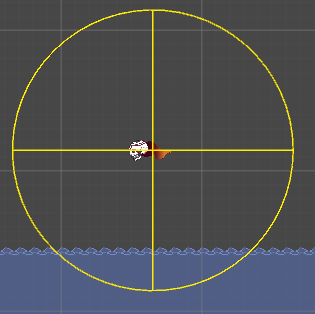
\includegraphics[width=0.4\textwidth]{03TrabajoRealizado/imagenes/EnemyRaycasting.png}
                    \caption{Ejemplo del área de acción del enemigo \textit{RedGhost}}
                    \label{fig:EnemyArea}
                \end{figure}
           
         \item \textbf{Cantidad de vida}: En el primer prototipo todos los enemigos
         eran derrotados por un único disparo, esto limitaba el factor de reto del
         juego al no ofrecer enemigos más resistentes al ataque del jugador. En el
         fin de ofrecer una nueva capa de complejidad a los enemigos se agrega a la
         clase \textit{Enemy} el atributo \textit{maxHealth} y \textit{healthAmount},
         estos atributos son los encargados de almacenar la máxima cantidad de vida
         que un enemigo puede tener y la vida actual de dicho enemigo (ver figura
         \ref{fig:EnemyAtributes}). La cantidad de
         vida sólo se actualiza cuando el enemigo es atacado por el jugador o cuando
         se reinicia el nivel. Para la actualización de la vida del enemigo se utiliza
         el comando \textit{Clamp} de la clase \textit{Math}, este comando permite
         especificar rangos con valores máximos y mínimos del resultado de operaciones,
         esto con la finalidad de que la vida actual del enemigo nunca sea cero y nunca
         sobrepase a su máximo de vida (ver figura \ref{fig:EnemyHealth}).
        
             \begin{figure}[h]
                    \centering
                    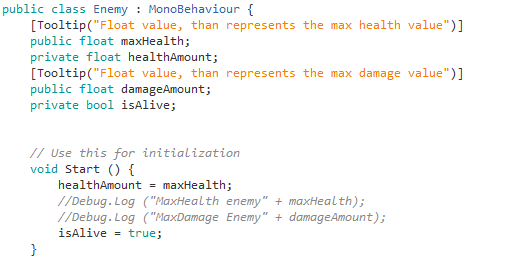
\includegraphics[width=0.6\textwidth]{03TrabajoRealizado/imagenes/EnemyClass.png}
                    \caption{Nuevos atributos para la clase \textit{Enemy}.}
                    \label{fig:EnemyAtributes}
            \end{figure}
            
            \begin{figure}[h]
                    \centering
                    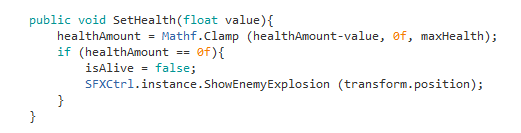
\includegraphics[width=0.6\textwidth]{03TrabajoRealizado/imagenes/EnemyClassMethodHealth.png}
                    \caption{Actualización de la cantidad de vida de la clase
                    \textit{Enemy}.}
                    \label{fig:EnemyHealth}
            \end{figure}
            
         \item \textbf{Cantidad de daño}: Al igual que con la cantidad de vida, los
         enemigos del primer prototipo infringen la misma cantidad de daño sin
         importar su tipo; por lo que para tener enemigos más y menos fuertes se agrega
         el atributo \textit{damageAmount}. Un enemigo puede infringir daño al jugador
         cada vez que toca al jugador o cuando dispara un ataque. Cada vez que un
         enemigo o un disparo enemigo choca con el jugador, el objeto enemigo manda
         a llamar el método \textit{SetHealth} del \textit{Player} y le envía como
         parámetro el valor de su atributo \textit{damageAmount}, seguido de un segundo 
         método
         de la clase \textit{Player} llamado \textit{EnemyNockBack}, este método es
         el encargado de la animación que indica que el jugador ha recibido daño (ver
         figura \ref{fig:PlayerGetsDamage}).
            
            \begin{figure}[h]
                \centering
                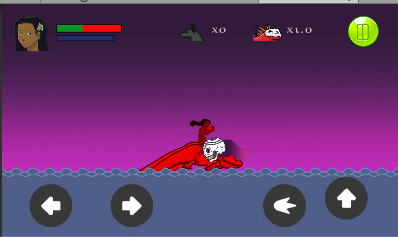
\includegraphics[width=0.4\textwidth]{03TrabajoRealizado/imagenes/EnemyRaycasting02.png}
                \caption{Ejecución de los métodos \textit{SetHealth} y \textit{EnemyNockBack} de la clase \textit{Player}, los cuales actualizan la cantidad de vida del jugador y muestran la animación de que el jugador ha recibido daño.}
                \label{fig:PlayerGetsDamage}
            \end{figure}
            
         \item \textbf{Girar horizontalmente}: En el primer prototipo el enemigo era
         incapaz de girar sus \textit{Sprite} y su ataque una vez que el jugador lo sobrepasaba como se ve en la figura \ref{fig:EnemyBack}. Utilizando la posición del enemigo y la posición del jugador dentro del área activa, el enemigo puede voltear su sprite y su ataque con base al valor de la distancia entre éste y el jugador:
         \begin{itemize}
             \item Si la posición del enemigo es mayor que las del jugador, el enemigo
             mantiene su orientación inicial.
             \item Si la posición del jugador es mayor que la del enemigo, el enemigo
             se voltea.
         \end{itemize}          

         Voltear un \textit{Sprite} no representa mayor problema en código; sin 
         embargo, el
         voltear un \textit{sprite} cuyo colisionador no es simétrico como el de 
         la figura
         \ref{fig:FixerCollider}. Esto puede representar un problema cuando se tiene
         que detectar colisiones, tal y como ocurre con los enemigos de tipo 
         \textit{RedGost} y
         \textit{PulpleGost}; para evitar alterar la detección de colisiones se 
         crea una nueva
         clase auxiliar llamada \textit{FixerCollider},  cuyo objetivo es ajustar 
         la posición
         del colisionador una vez que el personaje se gira como se puede observar en
         la figura \ref{fig:FixerCollider}.
        
         \begin{figure}[h]
                \centering
                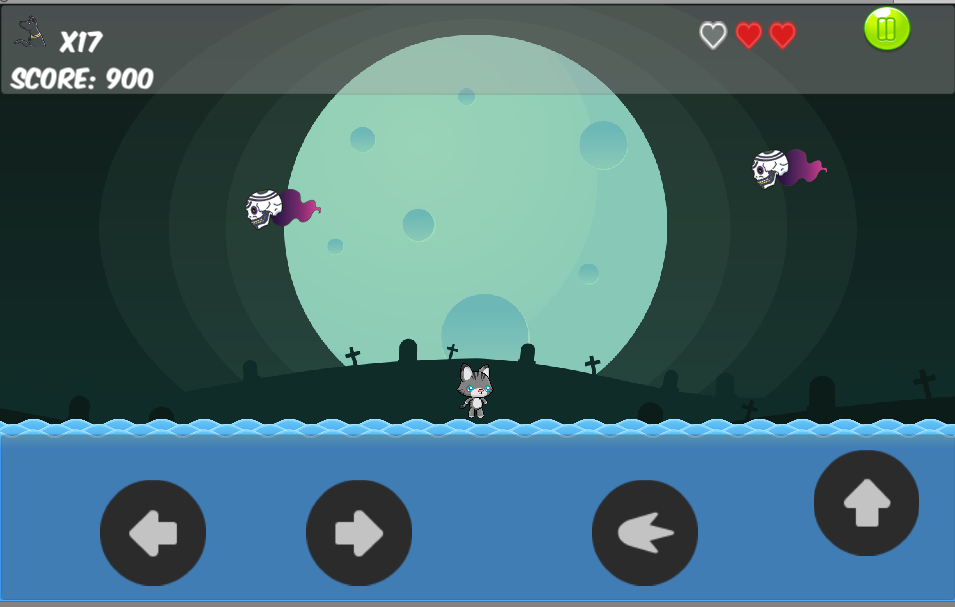
\includegraphics[width=0.4\textwidth]{03TrabajoRealizado/imagenes/voltearEnemigo01.png}
                \caption{En los primeros prototipos el enemigo es incapaz de girar su sprite y su ataque una vez que el jugador se coloca tras de éste.}
                \label{fig:EnemyBack}
        \end{figure}
        
        \begin{figure}[h]
              \centering
               \subfigure[ Ejemplo de un colisionador no simétrico respecto al \textit{sprite}.] {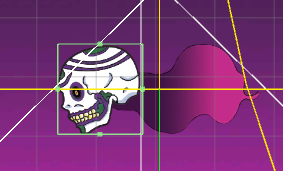
\includegraphics[width=0.3 \textwidth]{03TrabajoRealizado/imagenes/voltearEnemigo02.png}}
       
             \subfigure[Al girar el sprite de manera horizontal la posición del colisionador no se modifica]{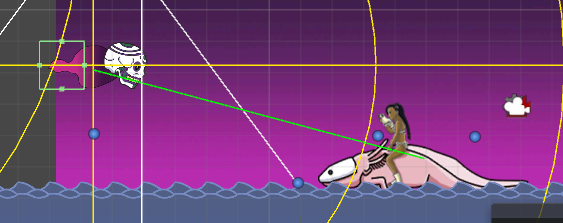
\includegraphics[width=0.3 \textwidth]{03TrabajoRealizado/imagenes/voltearEnemigo04.png}}
         
            \subfigure[Posición del colisionador modificada al emplear la clase \textit{FixerCollider}.] {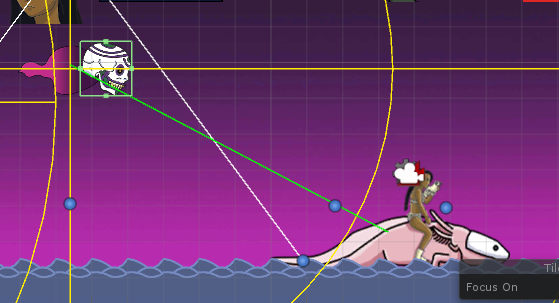
\includegraphics[width=0.3 \textwidth]{03TrabajoRealizado/imagenes/voltearEnemigo03.png}}
            
              \caption{Comportamiento del colisionador antes y después de la implementación de la clase \textit{FixerCollider}.}
              \label{fig:FixerCollider}
        \end{figure}
        
         \item \textbf{Trigger Collider}: En el primer prototipo el colisionador del
         enemigo tenía una configuración del tipo sólido lo que ocasionaba que cuando
         el enemigo chocaba con otro enemigo o con algún ataque enemigo este se
         estancara o fuera empujado por el objeto contra el que chocaba.
         Para corregir este comportamiento se configura el colisionador como uno de tipo
         trigger (ver figura \ref{fig:EnemyColliderTri}).  
            
            \begin{figure}[h]
                \centering
                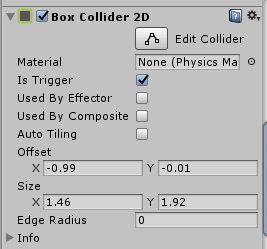
\includegraphics[width=0.3\textwidth]{03TrabajoRealizado/imagenes/Colisonador01.png}
                \caption{Configuración actual del colisionador de los enemigos.}
                \label{fig:EnemyColliderTri}
            \end{figure}    
        
         \item \textbf{Rigidbody2D}: Para evitar el comportamiento mencionado en el
         \textit{Trigger Collider} también fue necesario modificar la configuración
         del componente \textit{Rigidbody2D}, este componente pasa de estar en modo
         \textit{Dynamic} a modo \textit{Kinematic} lo que permite evitar que el objeto
         de juego reaccione conforme a las leyes físicas comunes.   
             
             \begin{figure}[h]
                \centering
                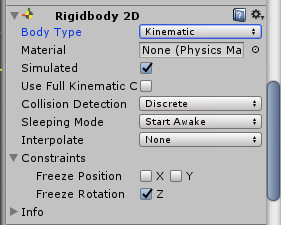
\includegraphics[width=0.3\textwidth]{03TrabajoRealizado/imagenes/Colisonador02.png}
                \caption{Configuración actual del componente \textit{Rigidbody2D} de
                los enemigos.}
                \label{fig:EnemyRigidBody}
            \end{figure}
    \end{itemize}

Para implementar cada uno de los patrones de movimiento de los enemigos es necesario
utilizar posiciones auxiliares que indiquen el límite del movimiento del personaje,
salvo en la clase Vulture ya que este explota al hacer contacto con el jugador. En la figura \ref{fig:JaguarCode} se puede observar el patrón de movimiento del enemigo de tipo jaguar expresado en código. Este comportamiento consiste en un movimiento recto horizontal de un punto A a un punto B y de regreso, haciendo una pausa en el movimiento cada vez que el jaguar ha alcanzado cualquiera de los puntos A o B (ver figura ).
\\
\par
            \begin{figure}[h]
                \centering
                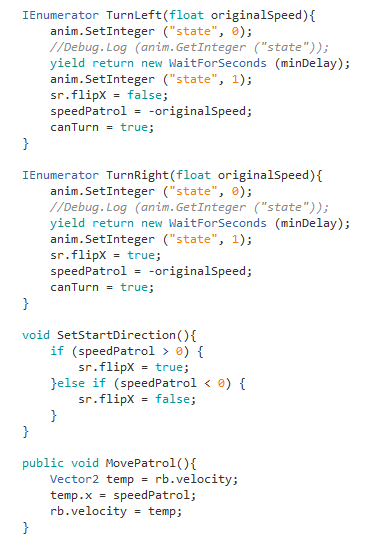
\includegraphics[width=0.3\textwidth]{03TrabajoRealizado/imagenes/PatronJaguar.png}
                \caption{Patrón de movimiento del enemigo tipo Jaguar expresado en
                código.}
                \label{fig:JaguarCode}
            \end{figure}
            
            \begin{figure}[h]
                \centering
                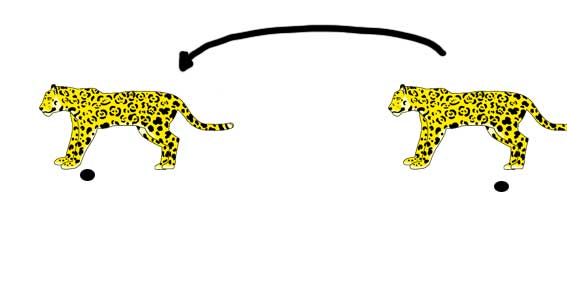
\includegraphics[width=0.3\textwidth]{03TrabajoRealizado/imagenes/saltoFelino.jpg}
                \caption{Patrón de movimiento del enemigo tipo Jaguar expresado en
                su comportamiento visual.}
                \label{fig:JaguarBeha}
            \end{figure}


Para resaltar la muerte de un enemigo se agrega un efecto especial de explosión
acompañado de un efecto de sonido para la explosión del personaje. Para esta
funcionalidad se implementa la clase \textit{SFXCtrl} y \textit{AudioCtrl} para 
manejar los efectos
de especiales y el sonido respectivamente, siendo estos los primeros controladores
en ser implementados.

\subsection{Implementando los enemigos jefes del juego}
Para la implementación de los enemigos jefes se reutilizan las configuraciones de los enemigos
normales referentes a las componentes \textit{Rigidbody2D} y \textit{Colisionador}, así como 
a la clase \textit{Enemy} para el manejo de vida y el uso de los efectos
de sonido y de explosiones para la muerte del jefe.
\\
\par
La lógica teórica tras los jefes del juego está inspirada por el jefe
\textit{Roxas} (ver figura \ref{fig:Roxas}) del juego \textit{Kingdom Hearts 2
Final Mix}. Dentro de \textit{Kingdom Hearts 2 Final Mix}, \textit{Roxas} es uno
de los jefes que requiere mayor habilidad de juego para ser derrotado, ya que a
diferencia del resto de los jefes de \textit{Kingdom Hearts 2 Final Mix}, el
patrón de ataque de \textit{Roxas} es totalmente aleatorio. Es decir, el jugador
puede saber en qué consiste cada uno de los ataques de este jefe, pero desconoce
el orden en el que estos serán ejecutados, salvo por algunos ataques que están
condicionados a una secuencia de ataque anterior.  Con los jefes del juego
\textit{Yolotl} sucede algo parecido, el jugador puede llegar a conocer lo tipos
de ataque que posee un jefe determinado pero la secuencia de ejecución de los
ataques está programada para que sea aleatoria, lo que puede generar experiencias
de juego muy sencillas o bastante retadoras para el jugador. El anterior
comportamiento se logra simulando una máquina de estados[referencia] 
con un arreglo de tipo booleano llamado \textit{whatCanDo}, en el cual solo un índice puede tener el
valor verdadero cada vez que se actualiza el estado y dependiendo del valor del
índice del valor verdadero será el ataque que ejecutará el enemigo. Después de
cada ataque el enemigo espera un tiempo determinado antes de asignar el siguiente
y ejecutarlo. Para ayudar al lector a comprender el funcionamiento de los jefes se
explica nuevamente usando como ejemplo al jefe \textit{Itzpapálotl} del nivel
cuatro. El jefe \textit{Iztpapálotl} cuenta con cuatro acciones:
    \begin{itemize}
        \item \textbf{\textit{WaitForAction:}} Espera un tiempo determinado y asigna
        un nuevo índice valor verdadero del arreglo de valores booleanos. Se activa
        si \textit{whatCanDo}[0] es verdadero.
        \item \textbf{\textit{shotFire}}: Dispara cuatro esferas de fuego que siguen
        al jugador y en caso de no chocar con este después de un tiempo se destruyen.
        Se activa si \textit{whatCanDo}[1] es verdadero.
        \item \textbf{\textit{useShell}}: Invoca un círculo de fuego que protege a
        \textit{Itzpapálotl} de cualquier daño, el escudo de fuego también puede
        infringir daño al jugador si hace contacto con éste. Se activa si
        \textit{whatCanDo}[2] es verdadero.
        \item \textbf{\textit{CreateButterflies}}: Invoca mariposas en tres puntos
        del campo, las mariposas también infringen daño al jugador y desaparecen
        después de un tiempo. Se activa si \textit{whatCanDo}[3] es verdadero.
    \end{itemize}
Al inicializarse el jefe \textit{Itzpapálotl whatCanDo}[0] es igual a cero. Por
lo que \textit{Itzpapálotl} ejecuta \textit{waitForAction}, al terminar la
ejecución de \textit{waitForAction}, \textit{whatCanDo}[0] es igual a falso y un nuevo
índice tiene ahora el valor verdadero. Supóngase ahora \textit{whatCanDo}[2] es
verdadero. \textit{Itzpapálotl} ejecuta \textit{useShell}, al terminar su
ejecución asigna \textit{whatCanDo}[2] como falso y asigna a \textit{whatCanDo}[0]
como verdadero. Nuevamente \textit{Itzpapálotl} espera unos segundos y actualiza
\textit{whatCanDo}. Por la naturaleza aleatoria de la actualización,
\textit{whatCanDo}[2] puede ser nuevamente verdadero o lo puede ser cualquier
otro índice exceptuando al 0 o a un número mayor que el índice máximo del
arreglo. En la figura se muestra la verificación de los valores de
\textit{whatCanDo} antes de la ejecución de cualquiera de los ataques que
tienen asignados. En la figura \ref{fig:EnemyMaquina} se muestra un ejemplo en
código de la maquina de estados del jefe \textit{Itzpapálotl}.
\\
\par
Por la forma en la que fue diseñado el comportamiento de la máquina de estados,
el nivel de dificultad que presente el jefe está dado en función de dos variables:
\textit{damageAmount} y \textit{timeBetweenAttacks}, correspondientes a la
cantidad de daño que el jefe puede infringir en el jugador y al tiempo que se
espera para actualizar los valores de \textit{waitForAction}. A mayor cantidad
de daño y menor tiempo de espera entre ataques, mayor será la dificultad para
derrotar al enemigo.

            \begin{figure}[h]
                \centering
                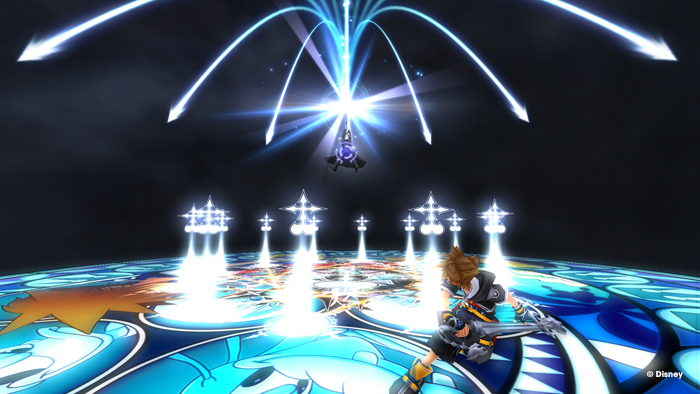
\includegraphics[width=0.5\textwidth]{03TrabajoRealizado/imagenes/RoxasBoss.jpg}
                \caption{\textit{Roxas} es el jefe más retador de \textit{Kingdom Hearts 2 Final Mix}. $ [Imagen] (2014)$ Recuperado de: \url{https://images.khinsider.com/2014\%20Uploads/05/Screenshots\%205-30/KHII_battle_03_EN\%20copy_1401446206.jpg}}
                \label{fig:Roxas}
            \end{figure}04R

            \begin{figure}[h]
                \centering
                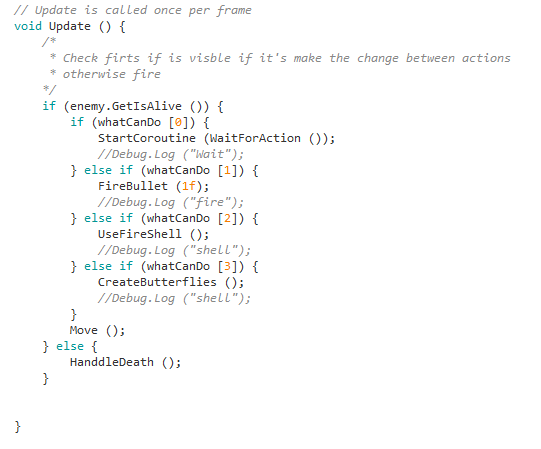
\includegraphics[width=0.5\textwidth]{03TrabajoRealizado/imagenes/ActualMaquinaJefe.png}
                \caption{Ejemplo de la máquina de estados del enemigo jefe.}
                \label{fig:EnemyMaquina}
            \end{figure}

\subsection{Implementando los ataques enemigos del juego}
Dentro del juego existen seis tipos de ataques enemigos:
    \begin{itemize}
        \item \textbf{Disparos con una trayectoria definida:} Este tipo de
        disparo sigue una trayectoria recta horizontal como se ve en la figura         
        \ref{fig:Enemyshot}.
        Para evitar la saturación de objetos dentro del juego, todos los disparos de
        este tipo se destruyen después de un tiempo. Para implementar este tipo de
        ataque se crea un \textit{GameObject} y se le agregan los siguientes
        componentes:
            \begin{itemize}
                \item \textbf{Collisionador:} El colisionador permite detectar si este
                ataque hace contacto con el \textit{Player} o con el suelo del nivel,
                en el primer caso se infringe daño al \textit{Player} y se destruye el
                \textit{GameObject}, en el segundo el \textit{GameObject} solo se
                destruye.
                \item \textbf{\textit{Rigidbody2D}}: El \textit{rigidbody2D} se
                configura
                con la opción \textit{kinematic} para evitar que el movimiento del
                disparo se vea afectado por la gravedad. Este componente permite en el
                código agregarle una velocidad al objeto.
                \item \textbf{\textit{DestryWithDelay}}: Componente creado por medio de
                la clase del mismo nombre, esta clase destruye al \textit{GameObject}
                que la contiene después de una cantidad determinada de tiempo.
                \item \textbf{\textit{EnemyBullet}}: Esta clase controla en la velocidad
                y dirección del movimiento del disparo, también tiene como atributo el
                daño que causa la bala y gestiona las colisiones del objeto.
            \end{itemize}
        Este tipo de disparo es empleado por los enemigos de tipo \textit{RedGost,
        Tepeyóllotl} y por \textit{Mictlantecuhtli}.
            
            \begin{figure}[h]
                \centering
                
\includegraphics[width=0.5\textwidth]{03TrabajoRealizado/imagenes/disparoTrayectoria.png}
                \caption{Ejemplo de un disparo de una trayectoria definida.}
                \label{fig:Enemyshot}
            \end{figure}
            
        \item \textbf{Disparos que siguen al jugador}: Este tipo de disparo sigue un
        comportamiento y configuración parecida al anterior con la diferencia que en
        este tipo el disparo seguirá al jugador hasta impactarse contra éste o
        destruirse después de un tiempo si no colisiona contra el jugador. Este
        comportamiento requiere que el disparo tenga una referencia a la posición del
        jugador para moverse hacia él, en la figura \ref{fig:FollowedShot}se puede ver
        la implementación de disco comportamiento en código. Este ataque es utilizado
        por los enemigos de tipo \textit{Mictlantecuhtli}, \textit{Tepeyóllotl},
        \textit{Itzpapálotl, Xochitonal} y \textit{Tlazolteolt}. Para todos estos
        enemigos el disparo tiene el mismo efecto que es el de infringir
        daño en el jugador; sin embargo, en el tipo de \textit{Tlazolteolt} este tipo de
        disparo también puede disminuir la cantidad de \textit{Tonalli} del Player.
            
            \begin{figure}[h]
                \centering
                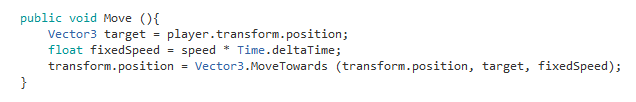
\includegraphics[width=0.5\textwidth]{03TrabajoRealizado/imagenes/disparoSigue.png}
                \caption{Implementación en código del comportamiento del disparo que sigue al jugador.}
                \label{fig:FollowedShot}
            \end{figure}        
        
        \item \textbf{Escudo de defensa que desaparece después de un tiempo}: Este
        ataque es efectuado por \textit{Itzpapálotl}. Al invocarse este escudo el
        enemigo no se ve afectado por los ataques del jugador. Este escudo no puede ser
        destruido y desaparece después de un tiempo que se invocó; este comportamiento
        se logra utilizando el método \textit{Invoke}, este método permite ejecutar
        métodos después de una cantidad de segundos; por lo que la desactivación se
        consigue mandando a llamar al método responsable de esto con \textit{Invoke}
        y asignando una cantidad determinada de segundos de espera.
        Inflige daño al jugador al hacer contacto con él.

        \item \textbf{Escudo de defensa que debe de ser destruido para desaparecer}:
        Ataque utilizado por \textit{Tlazolteolt}. Este escudo puede ser destruido
        por disparos del jugador y no desaparece al cabo de un tiempo. Al igual que el
        anterior protege al enemigo de los ataques del jugador e inflige daño si el
        jugador hace contacto con éste. Este tipo de escudo no cuenta con un método
        que lo desactive, en su lugar tiene una cantidad de vida determinada y que
        al llegar a cero, por efecto de los ataques del jugador, desaparece y reaparece
        hasta que el enemigo jefe lo vuelva a convocar.

        \item \textbf{Objetos que aparecen en posiciones cuya aparición tiene un tiempo
        de duración}: Este ataque es empleado por \textit{Itzpapálotl} y
        \textit{Mictlantecuhtli}. Cuando se activa provoca que se creen instancias del
        \textit{GameObject} que contiene la clase \textit{Butterfly}. Esta clase genera
        un movimiento vertical ascendente e inflige daño al jugador al hacer contacto
        con esta. La creación de estos \textit{GameObjects} se mantiene activa por un
        periodo de tiempo y después desactiva.Este funcionamiento se logra de una
        manera similar al comportamiento del escudo de defensa que desaparece después
        de un tiempo utilizando el método \textit{Invoke}. En la figura se puede
        observar la implementación en código de este tipo de ataque.  

        \item \textbf{Objetos que aparecen en posiciones de manera periódica}: Este
        ataque genera una lluvia de huesos o de piedras que le infringen daño al
        jugador una vez hacen contacto con este de lo contrario se destruyen al hacer
        contacto con el suelo. Para la creación de los objetos se utiliza el método
        \textit{Invoke} el cual controla la cantidad de \textit{GameObject} que se
        crean. Este ataque es utilizado por \textit{Mictlantecuhtli} y
        \textit{Tepeyóllotl}.
    \end{itemize}
 
\subsection{Implementando los obstáculos}
Una de las características de un juego de plataformas es la existencia de diferentes
obstáculos que el jugador debe de superar por medio de saltos\cite{Ref_JuegoDisenio}.
En \textit{Yolotl} se diseñaron e implementaron diferentes tipos de obstáculos
para ofrecer una variedad de retos al jugador, a continuación, se describe cada
uno de ellos y cómo fue que fueron implementados en el juego:
    \begin{itemize}
        \item \textbf{Plataforma que se mueve:} Es uno de los elementos más comunes de
        los juegos de plataforma, este   obstáculo consiste en una superficie de que
        se mueve de una posición a otra, ver figura \ref{fig:MovingPlatform}. dentro
        del juego se creó la clase \textit{MovingPlatform} para este tipo de obstáculo.
        \textit{MovingPlatform} tiene por atributos las posiciones a las que se moverá,
        velocidad a la que se moverá. Para su movimiento la clase hace uso de cuatro
        vectores de posiciones \textit{pos01, pos02, startPos} y \textit{nextPos}.
        \textit{Pos01} y \textit{pos02} son las posiciones límite que alcanzará la
        plataforma, \textit{startPos} es la posición hacia la que la plataforma inicie
        su movimiento inicial y \textit{nextPos} es la siguiente posición a la que se
        ira la plataforma una vez que haya alcanzado un límite. Manejar el
        comportamiento de las plataformas móviles con este sistema de posiciones
        permite que la plataforma pueda tener movimiento horizontal, vertical o diagonal
        sin la necesidad de reescribir código. Al igual que con los enemigos las
        plataformas de este tipo tienen un radio de área activa para evitar que su
        comportamiento se ejecute si no están visibles al jugador. Asignar el movimiento
        de la plataforma no es suficiente para su correcto funcionamiento, ya que
        cuando el movimiento de la plataforma es horizontal, ésta se desplaza sin el
        personaje ya que por sí misma no es capaz de asignarle un movimiento al jugador,
        por tal motivo fue necesario crear una nueva etiqueta para las plataformas
        llamada \textit{Platform} y asignar dos nuevos parámetros en las colisiones
        al jugador
        una para cuando entra en contacto con el colisionador de la plataforma y otra
        cuando sale. Cuando el jugador entra en contacto con el colisionador de la
        plataforma se le asigna un parentesco con la posición de la plataforma, lo
        que le permite seguir el movimiento de la plataforma, este parentesco se
        rompe cuando el jugador sale de la plataforma, en la figura
        \ref{fig:MovingPlatformCol} se puede ver esto en código. Adicionalmente,
        se utilizó el comando \textit{OnDrawGizmos} para dibujar la trayectoria de la
        plataforma a fin de facilitar la configuración de las plataformas móviles en la
        construcción de los niveles, ver figura \ref{fig:MovingPlatformWay}.
            
            \begin{figure}[h]
                \centering
                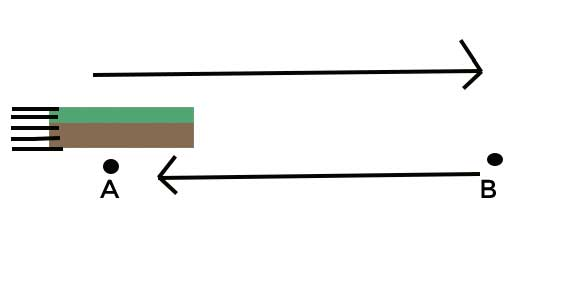
\includegraphics[width=0.5\textwidth]{03TrabajoRealizado/imagenes/plataformaMovil.jpg}
                \caption{Comportamiento de la plataforma que se mueve de manera visual.}
                \label{fig:MovingPlatform}
            \end{figure}
            
            \begin{figure}[h]
                \centering
                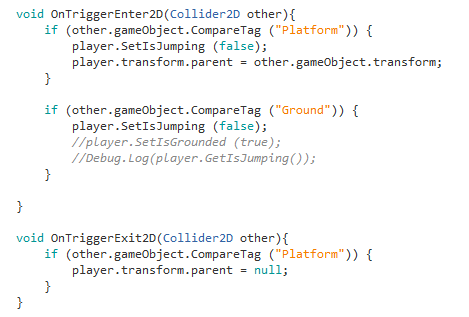
\includegraphics[width=0.5\textwidth]{03TrabajoRealizado/imagenes/plataformaColisiones.png}
                \caption{Gestión de la respuesta ante diferentes colisiones para
                garantizar el comportamiento de una plataforma que se mueve de manera
                horizontal.}
                \label{fig:MovingPlatformCol}
            \end{figure}
            
            \begin{figure}[h]
                \centering
                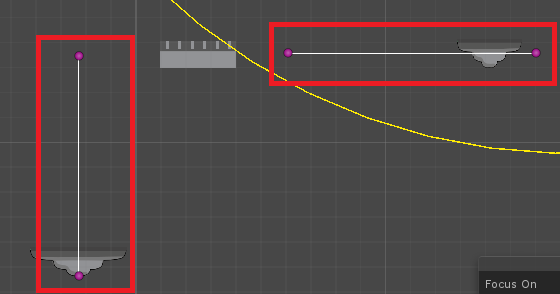
\includegraphics[width=0.5\textwidth]{03TrabajoRealizado/imagenes/plataformaConfig.png}
                \caption{Uso del método \textit{OnDrawGizmos} para visualizar la
                trayectoria de una plataforma que se mueve.}
                \label{fig:MovingPlatformWay}
            \end{figure}

        \item \textbf{Plataforma que cae}: Este tipo de plataforma se cae después de
        que el jugador se posiciona sobre ella. Para evitar que la plataforma caiga
        instantáneamente una vez que el jugador ha caído sobre ella, un tiempo de
        retraso se le asigna a la caída.

        \item \textbf{Plataforma con más de dos posiciones de control}: esta plataforma
        puede seguir patrones complejos movimiento como círculos, rectángulos o
        cuadrados. Su funcionamiento es similar a la plataforma que se mueve con la
        diferencia de que soporta más de dos posiciones de control; para esto se vale
        de un arreglo de posiciones en donde el atributo de \textit{nextPos} recorre
        todo el arreglo de posiciones y al llegar al último elemento del arreglo se
        le asigna el valor del primer elemento reiniciando el recorrido, ver figura .

        \item \textbf{Viento}: Ese obstáculo crea una corriente de viento que empuja
        al jugador hacia el vacío, ver figura . Para crear este obstáculo se crean
        tres clases: \textit{PushingObstacle}, \textit{WindCreator} y
        \textit{WindHelper}. La primera controla el movimiento del viento a crear.
        La segunda crea el viento por periodos de tiempo dejando un tiempo de
        inactividad para que el jugador pueda pasar y la tercera activa al creador
        de viento cuando el jugador entra en el área activa del obstáculo, cada clase
        está instanciada en un \textit{GameObject} diferente. En un principio solo
        existían las clases \textit{PushingObstacle} y \textit{WindCreator}, lo que
        provoca que el creador de viento cree viento aun cuando el obstáculo no es
        visible para el jugador; esto ocasiona la creación de muchos
        \textit{GameObjects} innecesarios para el viento, por tal motivo se crea la
        clase \textit{WindHelper} para controlar la activación del
        creador de viento.  Para definir los periodos de creación de viento y de pausa
        de viento es necesario probar diferentes valores para asignar los tiempos de
        creación y de pausa del viento. Luego de varias pruebas se definen los
        siguientes tres valores: 4 para el tiempo activo de creación, 8 para el tiempo
        de pausa de viento y 0.4 para la pausa entre creación de instancias de viento.

        \item \textbf{Estalagmitas}: Este obstáculo se cae e inflige daño en el
        jugador cuando éste pasa por debajo del obstáculo, ver figura .  Para
        implementar este obstáculo se crean dos clases: \textit{Stalagmite} y
        \textit{StalagmiteCtrl}. La primera clase gestiona la caída del objeto y el
        daño que le infringe al jugador si choca con este o la destrucción del objeto
        en caso de que choque con el suelo. La segunda clase se encarga de indicarle
        a la clase \textit{Stalagmite} que el jugador va a pasar bajo de ella para que
        inicie su caída. En la figura \ref{fig:StalagmiteConf} se puede ver la
        configuración de ambos objetos dentro de un nivel.
        
            \begin{figure}[h]
                \centering
                \includegraphics[width=0.3\textwidth]{03TrabajoRealizado/imagenes/StalagmiteConfig.png}
                \caption{Configuración de los diferentes \textit{GameObjects} que
                conforman el obstáculo estalagmita.}
                \label{fig:StalagmiteConf}
            \end{figure}
        
        \item \textbf{Obstáculo que hace daño}: este obstáculo infringe daño al jugador
        cuando éste hace contacto con él y no puede ser destruido por el mismo. Este
        tipo de obstáculo se puede encontrar en el segundo nivel en la etapa de
        plataforma. Para su implementación se crea la clase \textit{DamageObstacle} y 
        esta
        gestiona el daño que infringe el obstáculo pudiendo generar obstáculos que
        causen más o menos daños que otros.

        \item \textbf{Xólotl en su forma Colibrí}: Este obstáculo tiene un
        comportamiento parecido a la plataforma con más de dos posiciones de
        control anteriormente descrita, con la diferencia de que su movimiento
        describe una línea y no un circuito cerrado; por otro lado, al morir el
        jugador este obstáculo regresa a su posición inicial. Este obstáculo aparece
        únicamente en el nivel 6, donde el jugador deberá cruzar distintos segmentos
        del mapa sobre este obstáculo y tendrá que vencer a los enemigos que vayan
        apareciendo para avanzar, ver figura .
    \end{itemize}

\subsection{Implementando los ítems y los objetos coleccionables}
Las últimas clases actoras en ser implementadas fueron los ítems, los objetos
coleccionables y los puntos de guardado, ya que en el caso de los ítems y los
puntos de guardado se necesitaba que el jugador sufriera daño, gastara
\textit{tonalli} o muriera ya fuera a causa de enemigos u obstáculos.
\\
\par
Dentro del juego existen dos tipos de ítems: Los que recuperan cantidad de vida y
los que recuperan cantidad de tonalli. Ambos tienen un funcionamiento similar: como
atributos sus respectivas clases tienen una cantidad de lo que van a restaurar
(sea \textit{tonalli} o vitalidad), al hacer contacto con el jugador le incrementan
dicho atributo en la cantidad que tienen asignada y se destruyen mostrando un
efecto de brillos y un efecto de sonido.
\\
\par
En lo que se refiere a los objetos coleccionables dentro del juego se crea la
clase CollectableObjects, clase encargada de destruir los objetos coleccionables
una vez que el jugador los ha tocado, dejando la tarea de actualizar el marcador
al jugador. Para poder lograr la actualización del atributo \textit{score} del
\textit{Player} se asignaron etiquetas para los objetos coleccionables y dependiendo
de dichas etiquetas se gestiona la actualización de los marcadores, esto debido a que
la función de los objetos coleccionables depende directamente del nivel en el que
se encuentre el jugador; por ejemplo, para los perros que aparecen en el segundo
nivel, hacer contacto con uno de ellos no solo actualiza el marcador sino también
incrementa el poder que tendrá el Jefe de este nivel, por lo tanto
la actualización visual del marcador deberá incluir cuantos perros se han tocado
y en cuanto se ha incrementado el poder del jefe(ver figura
\ref{fig:CollectableObjects}); mientras que en el nivel 4, los coleccionables
son llaves y su función es la de desbloquear la transición al siguiente nivel
solo si se han juntado todas las llaves; visualmente esta actualización solo
requiere de la actualización de un elemento en pantalla (ver figura 
\ref{fig:CollectableObjects}). Para solucionar esto se crearon dos etiquetas 
para cada tipo de coleccionable: \textit{CollectableDog} y 
\textit{CollectableKey}.  Dejando al gestor de colisiones de la clase 
\textit{Player} verificar por medio de la etiqueta de qué tipo de coleccionable 
se trata e invoca al controlador de la interfaz gráfica de los marcadores del 
juego o \textit{HUB}.
            
            \begin{figure}[h]
              \centering
               \subfigure[El marcador referente a los perros se encuentra en cero, ya
               que el jugador no ha tocado ninguno de estos.] {\includegraphics[width=0.3 \textwidth]{03TrabajoRealizado/imagenes/InterfazJuego06.png}}
       
             \subfigure[Al tocar un perro el marcador referente al conteo de ellos se actualiza junto al del poder del jefe.]{\includegraphics[width=0.3 \textwidth]{03TrabajoRealizado/imagenes/InterfazJuego07.png}}
            
              \caption{Interacción entre el jugador y los objetos coleccionables del nivel.}
              \label{fig:CollectableObjects}
        \end{figure}

\subsection{Implementación de los puntos de guardado}
Los puntos de guardado o \textit{checkpoints} son los actores encargados de
hacer aparecer al jugador en una posición del nivel una vez que éste haya muerto,
evitando que el jugador pierda su progreso dentro del nivel. Un
\textit{checkpoint} se activa cuando el jugador hace contacto con éste. La
funcionalidad de este actor está dada por la clase \textit{CheckPoint}, esta clase
tiene como atributos(ver figura \ref{fig:CheckAtri}):

\begin{itemize}
    \item \textit{\textbf{isActive}}: Atributo booleano. Cuando es verdadero indica
    que el jugador  ha pasado por el checkpoint. Solo puede haber un único checkpoint
    activo.
    \item \textit{\textbf{CheckPointsList}}: Arreglo de GameObjects que instancian
    la clase CheckPoint.
\end{itemize}

Cuando el jugador entra en contacto con el \textit{checkPoint}, éste manda a
llamar el método \textit{ActivateCheckPoint}, este método toma todos los
elementos que hay en  \textit{CheckPointsList} y vuelve su atributo
\textit{isActive} falso, después vuelve verdadero el atributo \textit{isActive}
del \textit{checkPoint} que fue tocado por el jugador. Cuando el jugador muere
se manda a llamar el  método \textit{GetActivePosition}, este método busca el
\textit{checkPoint} activo y revive al jugador en esa posición. En la figura
\ref{fig:CheckMethod} se muestran los métodos de esta clase.

Existen dos tipos de \textit{checkPoints}:
    \begin{itemize}
        \item \textbf{\textit{CheckPoint} vacío}: este \textit{checkPoint} no 
        tiene ningún
        \textit{sprite} asignado y se encuentra al inicio del nivel. Está activo 
        por defecto
        y si el jugador muere sin antes tocar algún otro \textit{checkPoint}, la
        posición de este \textit{checkPoint} es donde aparecerá al revivir.
        \item \textbf{\textit{CheckPoint} normal}: Este \textit{checkPoint} tiene un
        búho como \textit{sprite} y una animación para cuando el jugador interactúa con
        él.
    \end{itemize}
    
\begin{figure}[h]
                \centering
                \includegraphics[width=0.3\textwidth]{03TrabajoRealizado/imagenes/checkpoint.png}
                \caption{Atributos de la clase \textit{CheckPoint}}
                \label{fig:CheckAtri}    
\end{figure}

\begin{figure}[h]
                \centering
                \includegraphics[width=0.3\textwidth]{03TrabajoRealizado/imagenes/checkpointmethods.png}
                \caption{Métodos de la clase \textit{CheckPoint}}
                \label{fig:CheckMethod}    
\end{figure}

\subsection{Cierre del sprint}
Al término de este \textit{sprint} se cuenta con todos los \textit{Assets} de
los actores organizados en diferentes carpetas como \textit{Player, Obstacles, Enemies},
etc. Este \textit{sprint} se cierra con éxito y deja todos los elementos listos
para la construcción de las clases controladoras.


\subsection{Sprint plan 7}
\subsubsection{SprintID}
07
\subsubsection{Inicio}
29 Enero 2018
\subsubsection{Fin}
18 Febrero 2018
\subsubsection{Meta}
Nivel 7
\subsubsection{Porcentaje}
El 16\% 


\subsubsection{FeatureID}
07
\subsubsection{Nombre}
N7
\subsubsection{Estado}
Planeado
\subsubsection{SprintID}
07
\subsubsection{Comentarios}
-


\subsection{Sprint backlog 7}
\subsubsection{Sprint # backlog}
07
\subsubsection{Tareas}
14
\subsubsection{Tendencia}
0
\subsubsection{Esfuerzo restante}
56
\subsubsection{Tendencia actual}
-
\subsubsection{Progreso ideal}
14
\subsubsection{Tareas restantes}
14
\subsubsection{Nombre de la tarea}
n7
\subsubsection{FeatureID}
07
\subsubsection{Miembro}
Rocío
\subsubsection{Rol}
Desarrollo
\subsubsection{Estado}
Planeado
\subsubsection{Esfuerzo}
14



\subsection{Task Slips 9}


\subsubsection{FeatureID}7
\subsubsection{Nombre}Maqueta
\subsubsection{Tarea}Realizar maqueta del nivel completo
\subsubsection{Miembro}Rocío
\subsubsection{Esfuerzo estimado}1
\subsubsection{Terminado}si
\subsubsection{Restante}0


\subsubsection{FeatureID} 7
\subsubsection{Nombre} Enemigos
\subsubsection{Tarea} Realizar el comportamiento de los enemigos o cualquier otra acción necesaria dentro del nivel
\subsubsection{Miembro} Rocio
\subsubsection{Esfuerzo estimado} 5
\subsubsection{Terminado} sí
\subsubsection{Restante} 0


\subsubsection{FeatureID} 7
\subsubsection{Nombre} Arte 1
\subsubsection{Tarea} Crear vista de los personajes
\subsubsection{Miembro} Rocío
\subsubsection{Esfuerzo estimado} 2
\subsubsection{Terminado} sí
\subsubsection{Restante} 0



\subsubsection{FeatureID} 7
\subsubsection{Nombre} Arte 2
\subsubsection{Tarea} Crear el diseño de los obstáculos
\subsubsection{Miembro} Rocío
\subsubsection{Esfuerzo estimado} 2
\subsubsection{Terminado} sí
\subsubsection{Restante} 0


\subsubsection{FeatureID} 7
\subsubsection{Nombre} Arte 3
\subsubsection{Tarea} Crear el diseño de los items
\subsubsection{Miembro} Rocio
\subsubsection{Esfuerzo estimado} 2
\subsubsection{Terminado} sí
\subsubsection{Restante} 0

\subsubsection{FeatureID} 7
\subsubsection{Nombre} Boss 1
\subsubsection{Tarea} Diseñar la máquina de estados del enemigo principal del nivel
\subsubsection{Miembro} Rocio
\subsubsection{Esfuerzo estimado} 2
\subsubsection{Terminado} sí
\subsubsection{Restante} 0

\subsubsection{FeatureID} 7
\subsubsection{Nombre} Boss 2
\subsubsection{Tarea} Crear la máquina de estados del enemigo principal del nivel
\subsubsection{Miembro} Rocio
\subsubsection{Esfuerzo estimado} 2
\subsubsection{Terminado} sí
\subsubsection{Restante} 0

\subsection{Octavo \textit{sprint} de producción}
En este \textit{sprint} se implementa en código la funcionalidad de todos los 
elementos controladores del juego y sus auxiliares, exceptuando a los 
controladores de los niveles ya que éstos se desarrollarán en el décimo 
\textit{sprint} dado que se requieren los niveles terminados para comprobar su 
funcionalidad.

\subsubsection{Controlador de Audio}
Este controlador es el encargado de gestionar los efectos de sonido del 
juego. Logra su funcionamiento con ayuda de la clase controladora 
\textit{AudioCtrl} y de la clase auxiliar \textit{PlayerAudio}. 
\\
\par
La clase \textit{PlayerAudio} está compuesta de los atributos del tipo 
\textit{AudioClip}. Por convención los archivos de audio que \textit{Unity} 
soporta pueden ser del tipo \textit{MP3}, \textit{OGG}, \textit{WAV}, entre 
otros, en relación a tamaño del archivo y calidad de audio se opta por utilizar 
los archivos de tipo \textit{OGG}. Para la importación de los archivos de audio 
se elige la configuración que se muestra en la figura \ref{fig:AudioClipConfi}, 
ya que ésta se disminuye el tiempo de carga de los audios y el espacio en 
memoria de almacenamiento que utilizan dentro de la aplicación. 
\textit{PlayerAudio} contiene cinco pistas de audio correspondientes a los 
efectos de sonido cuando: 
	\begin{itemize}
		\item El jugador hace contacto con un objeto coleccionable, como una 
		llave o un \textit{xoloitzcuintle}.
		\item El jugador hace contacto con un ítem.
		\item El jugador dispara \textit{tonalli}.
		\item Un enemigo es destruido.
		\item El jugador muere.
	\end{itemize}	 

\textit{PlayerAudio} se vale de la serialización para su funcionamiento(ver 
figura \ref{fig:PlayerAudio}), esta clase funge como un organizador de elementos 
para su visualización en el \textit{GameInspector}, como se ve en la figura 
\ref{fig:PlayerAudioConf}.   

	\begin{figure}[h]
		\centering
		\includegraphics[height=0.15 \textheight]{03TrabajoRealizado/imagenes/playerAudioConfig.png}
		\caption{Configuración de la importación de los archivos de audio.}
		\label{fig:AudioClipConfi}
	\end{figure}

	\begin{figure}[h]
		\centering
		\includegraphics[height=0.15 \textheight]{03TrabajoRealizado/imagenes/playerAudio.png}
		\caption{Serialización de la clase \textit{PlayerAudio}}
		\label{fig:PlayerAudio}
	\end{figure}


	\begin{figure}[h]
		\centering
		\includegraphics[height=0.1 \textheight]{03TrabajoRealizado/imagenes/audioCtrlGameInsp.png}
		\caption{Atributos organizados en el \textit{GameInspector} gracias a la serialización de la clase \textit{PlayerAudio}.}
		\label{fig:PlayerAudioConf}
	\end{figure}

Por su parte la clase \textit{AudioCtrl} tiene como atributos la clase 
\textit{PlayerAudio}, un vector de tres dimensiones para la posición del 
personaje que mande a llamar los métodos que invocan los audios y una instancia 
de la misma clase \textit{PlayerAudio} para la perseverancia de datos. Los 
métodos que contiene la clase son para invocar determinado audio, para esa 
funcionalidad se utiliza el método \textit{PlayClipAtPoint}, el cual necesita 
como atributos un objeto de tipo \textit{AudioClip} y un vector de tres 
dimensiones. Cada método que invoca un efecto de audio es mandado a llamar en la 
parte del código que implementa dicha funcionalidad, por ejemplo en el método 
\textit{SetHealth} del la clase \textit{Enemy} se agrega la linea de código que 
invoca el audio para la destrucción de un Enemigo en donde se maneja la muerte 
del enemigo. En la figura se pueden ver los atributos y los métodos de la clase 
\textit{AudioCtrl}.  

	\begin{figure}[h]
		\centering
		\includegraphics[height=0.3 \textheight]{03TrabajoRealizado/imagenes/audioCtrl.png}
		\caption{Atributos y métodos de la clase \textit{AudioCtrl}.}
		\label{fig:AudioCrl}
	\end{figure}

\subsubsection{Controlador de Diálogos}\label{ControladorDialogo}
Este controlador se emplea en la cinemáticas del juego.El controlador de 
Diálogos se vale de cuatro clases para su funcionamiento: 
\textit{Dialogue}, \textit{Dialogues}, \textit{DialogueFile} y 
\textit{DialogueCtrl}. 
\\
\par
Las clases \textit{Dialogue} y \textit{Dialogues}, son clases de tipo auxiliar. Ambas clases son serializadas y el objetivo de ellas es el de organizar la información en el \textit{GameInspector}. La clase \textit{Dialogue} tiene como atributos un \textit{string} para almacenar el nombre del personaje al que pertenece el dialogo y una lista de tipo \textit{string} para los diálogos. Por su parte la clase \textit{Dialogues} tiene como atributo una lista de tipo \textit{Dialogue}. El objetivo de la clase \textit{Dialogues} es la de almacenar todos los diálogos de la cinemática. En la figura \ref{fig:Dialogues} se puede ver la definición de las clases \textit{Dialogue} y \textit{Dialogues}.
\\
\par
La clase \textit{DialogueFile} se encarga de la gestión de los diálogos, al contenerlos y activar la visualización de los mismos por medio de la clase \textit{DialogueCtrl}. 
\\
\par 
La clase \textit{DialogueCtrl} se encarga de la visualización de los diálogos 
dentro de la escena. Por tal motivo parte de sus atributos son 
\textit{GameObjects} del tipo \textit{Text} de la \textit{UI}. La clase 
\textit{DialogueCtrl} visualiza los diálogos tomando el contenido de la clase 
\textit{Dialogue} y extrayendo elemento por elemento. De cada elemento extraído 
se obtiene su lista de diálogos y se almacena esta lista en un \textit{Queue} y 
se muestra en pantalla cada dialogo. La transición entre diálogos se hace si el 
jugador oprime el botón de salto, ver figura \ref{fig:NextDialogueBottom}. Una 
vez que el controlador ha mostrado todos los diálogos de un elemento. Los 
diálogos se visualizan por medio de una animación que nuestra carácter por 
carácter, en la figura \ref{fig:DialoguesCtrl} se muestra el método encargado de 
mostrar esta animación.   

	\begin{figure}[h]
		\centering
		\includegraphics[height=0.3 \textheight]{03TrabajoRealizado/imagenes/dialogueFile.png}
		\caption{Serialización de las clases \textit{Dialogue} y \textit{Dialogues}.}
		\label{fig:Dialogues}
	\end{figure}

	\begin{figure}[h]
		\centering
		\includegraphics[height=0.2 \textheight]{03TrabajoRealizado/imagenes/DialogueOnScreen.png}
		\caption{La transición entre diálogos se hace si el jugador oprime el 
		botón de salto, este botón es el que se encuentra encerrado en rojo.}
		\label{fig:NextDialogueBottom}
	\end{figure}

	\begin{figure}[h]
		\centering
		\includegraphics[height=0.15 \textheight]{03TrabajoRealizado/imagenes/dialogueController02.png}
		\caption{El método \textit{TypeSentences} es el encargado de animar el texto de los diálogos al mostrarlos en pantalla}
		\label{fig:DialoguesCtrl}
	\end{figure}

\subsubsection{Controlador de los datos del juego}
El controlador de datos del juego es el encargado de gestionar los datos 
relacionados al progreso del jugador, es decir los niveles desbloqueados, la 
cantidad de vida, la cantidad de \textit{tonalli}, el marcador y la cantidad de 
daño que hacen los ataques del jugador. Para su funcionamiento, este controlador 
se vale de las clases \textit{GameData} y \textit{GameDataCtrl}.
\\
\par
La clase \textit{GameData}, es una clase de tipo auxiliar y su función es la de 
serializar los datos que se van a almacenar en el archivo de los datos del 
juego, ver figura \ref{fig:GameData}. Por su naturaleza esta clase solo contiene 
la definicion de los atributos y sus \textit{getters} y \textit{setters}. 
\textit{Unity} maneja un tipo de archivo binario que permite la codificación de 
los datos para evitar que estos sean modificados por el jugador.
\\
\par
La clase \textit{GameDataCtrl} es la encargada de gestionar la creación del 
archivo, el cargado de la información y de salvar el progreso del jugador. Esta 
clase se debe de encontrar presente en todas las escenas del juego, ya que de 
los datos que ésta obtiene se inicializan los valores de la clase 
\textit{Player} y se verifican de los niveles disponibles. \textit{Unity} 
destruye todos los datos de una escena una vez que sale de ésta y crea una 
nueva, por lo que en cada escena se debería crear una instancia de la clase 
\textit{GameDataCrl}. Para evitar que se desperdicien recursos en el proceso de 
creación y destrucción de las instancias de la clase \textit{GameDataCrl} se 
recurre al patrón de diseño\textbf{ \textit{Singleton}}. El patron de diseño 
\textit{Singleton} garantiza que exista solo una instancia de una clase, lo que 
para el caso particular de \textit{Unity} se traduce en persistencia de la 
información entre escenas. En la figura \ref{fig:GameDataCtrl} se puede observar 
como se logra el comportamiento de un \textit{singleton} al agregar el método 
\textit{DontDestroyOnLoad}. El uso de un \textit{sigleton} hace que se tenga una 
configuración especial para el \textit{GameObject} que contenga a esta clase y 
garantizar que se tenga una única instancia. El \textit{GameObject} que contenga 
a la clase \textit{GameDataCtrl} debe de estar únicamente en la escena del menú 
principal y no debe de encontrarse en ninguna otra. Para probar el 
funcionamiento de los niveles del juego se puede tener tener un 
\textit{GameObject} que contenga a la clase \textit{GameDataCtrl} en dichas 
escenas pero es importante que cuando se construya la \textit{apk} del juego, 
todos estos \textit{GameObjects} se desactiven o se eliminen para evitar crear 
conflictos por múltiples instancias de la clase \textit{GameDataCtrl}.  

	\begin{figure}[h]
		\centering
		\includegraphics[height=0.15 \textheight]{03TrabajoRealizado/imagenes/GameData.png}
		\caption{Los atributos de la clase \textit{GameData} corresponden a los 
		datos que se guardaran en el archivo del progreso del juego por lo que 
		estos atributos se encuentran serializados}
		\label{fig:GameData}
	\end{figure}   
	
	\begin{figure}[h]
		\centering
		\includegraphics[height=0.2 \textheight]{03TrabajoRealizado/imagenes/gameDataCtrl.png}
		\caption{Inicialización de la clase \textit{GameDataCtrl} para 
		garantizar el patrón de diseño \textit{Singleton}.}
		\label{fig:GameDataCtrl}
	\end{figure}

\subsubsection{Controlador de fin de la partida}
El controlador de fin de partida funciona a partir de la clase 
\textit{GameOverCtrl} y de un \textit{GameObject} de tipo \textit{Panel}. La 
logica detras este controlador es la siguiente, en el \textit{Panel} se 
contienen los botones que tienen la funcionalidad de la interfaz que se muestra 
cuando el jugador ha muerto dentro del juego, ver figura 
\ref{fig:GameOverInterfaz}. La interfaz de fin de partida esta compuesta de tres 
botones uno para reiniciar la partida, otro para volver al menú de selección de 
nivel y el tercero para salir de la aplicación. La clase \textit{GameOverCtrl} 
se encarga de la funcionalidad de los botones y de hacer aparecer el 
\textit{panel} cuando el jugador es derrotado. En la figura 
\ref{fig:GameOverCtrl} se pueden observar los métodos de la clase \textit{GameOverCtrl}. 

	\begin{figure}[h]
		\centering
		\includegraphics[height=0.2 \textheight]{03TrabajoRealizado/imagenes/GameOverPanel.png}
		\caption{Interfaz que aparece cuando el jugador ha muerto dentro del juego para indicar que ha perdido.}
		\label{fig:GameOverInterfaz}
	\end{figure} 
	
	\begin{figure}[h]
		\centering
		\includegraphics[height=0.2 \textheight]{03TrabajoRealizado/imagenes/GameOverCtrl.png}
		\caption{Métodos de la clase GameOverCtrl}
		\label{fig:GameOverCtrl}
	\end{figure} 

\subsubsection{Controlador de la barra de vida y de \textit{tonalli} del jugador}
Este controlador se encarga de actualizar gráficamente la cantidad de vida y 
\textit{tonalli} con la que cuenta el jugador. Para la funcionalidad de este 
controlador se implementa un \textit{Panel} \textit{GameObject} para que 
contenga las barras de vida y tonalli del jugador del jugador. Las barras de 
vida y de tonalli se crean usando \textit{UI GameObjects} de tipo 
\textit{Image}. Para la barra de vida se emplean tres \textit{UI GameObjects} de 
tipo \textit{Image}:  
	\begin{itemize}
		\item \textit{Health}: de color verde, que representa la cantidad de 
		vida del jugador.
		\item \textit{Damage}: De color rojo, representa la cantidad de daño que 
		recibe el jugador, es del mismo tamaño que \textit{Health}.
		\item \textit{BarHealth:} De color negra, es ligeramente de mayor tamaño 
		que las dos anteriores y funge como borde para la barra de vida. Ver figura  \ref{fig:HealthBar}.
	\end{itemize}
La actualización de la barra de vida se consigue redimensionando el tamaño de 
\textit{Health}, Unity cuenta con el método \textit{localScale} que permite 
ajustar la dimensión de un \textit{GameObject}. \textit{LocalScale} requiere 
como argumento un vector de dos dimensiones para indicarle si se hará un ajuste 
horizontal o vertical del objeto, este método toma el 1 como la máxima dimensión 
del objeto por lo que si se quisiera que el la barra de vida se redujera a la 
mitad, se tendría que enviar como argumento al método un vector de $(0.5, 1)$. 
Para el valor en $x$ de la escala a la que se va a redimensionar \textit{Health} 
basta con dividir la cantidad actual de vida entre la cantidad máxima, es decir 
$health/maxHealth$. Para actualizar la barra de tonalli se requiere del mismo 
método. La clase \textit{HealthBar} es la encargada de gestionar el 
redimensionamiento de las barras de vida y de tonalli. Sus métodos 
\textit{UpDateHealthBar} y \textit{UpDateTonallithBar} son llamados en la clase 
\textit{Player} en los métodos \textit{SetHealt} y \textit{SetTonalli}, métodos 
encargados de actualizar la cantidad de vida y de \textit{tonalli} 
respectivamente. 

	\begin{figure}[h]
		\centering
		\includegraphics[height=0.1 \textheight]{03TrabajoRealizado/imagenes/attributesBar.png}
		\caption{Barras de vida y \textit{tonalli}.}
		\label{fig:HealthBar}
	\end{figure} 
	
\subsubsection{Controlador del panel de marcadores}
El controlador del panel de marcadores es el encargado de actualizar gráficamente cuantos objetos coleccionables ha juntado el jugador dentro de un nivel, ya sean llaves o \textit{xoloitzcuintles}, ver figura \ref{fig:HUB}. Para implementar la actualización gráfica de los marcadores ser crea un \textit{panel} \textit{GameObject} para contener los iconos de los objetos coleccionables y el texto que proporciona la información de los mismos. La clase \textit{HUBCtrl} es encargada de actualizar el texto referente a los marcadores; para tal funcion se vale de dos métodos:

	\begin{itemize}
		\item \textit{\textbf{UpDateDogScore:}}responsable de actualizar el conteo de \textit{xoloitzcuintles} y del poder de \textit{Xochitonal} en el segundo nivel.
		 \item \textit{\textbf{UpDateKeys:}} encargado de actualizar la cantidad de llaves colectadas en el cuarto nivel.
	\end{itemize}	 
	
	Estos métodos son mandados a llamar por la clase \textit{Player} en su método \textit{OnTriggerEnter2D}, ya que este es el que gestiona las reacciones del jugador y del juego ante las colisiones del jugador.

	\begin{figure}[h]
		\centering
		\includegraphics[height=0.05 \textheight]{03TrabajoRealizado/imagenes/HUB.png}
		\caption{Panel del marcador correspondiente al nivel 4.}
		\label{fig:HUB}
	\end{figure} 
	
\subsubsection{Controlador de pausa en el juego}
Este controlador permite pausar el nivel que se esta jugando al oprimir el botón 
de pausa que se encuentra en la esquina superior derecha de la pantalla, ver 
figura \ref{fig:PausedFuctionality}. Para implementar esta funcionalidad se 
agrega el botón de \textit{pausa} al panel de marcadores y se crea un nuevo 
panel parecido al de fin de partida con la diferencia que en lugar del botón de 
reintentar partida se pone el botón de quitar pausa del juego, ver figura 
\ref{fig:PausedFuctionality}. Dado que dos de los botones tienen la misma 
funcionalidad que el panel de fin de partida, los botones para salir de la 
aplicación y para ir al menu de selección de nivel toman la funcionalidad del 
\textit{GameOverCtrl}; mientras que el botón de pausa y de botón para quitar la 
pausa del juego toman su funcionalidad de la clase \textit{PauseCtrl}. La 
funcionalidad de \textit{PauseCtrl} se basa en el flujo del tiempo de la 
partida. \textit{Unity} permite controlar la velocidad de la partida con el 
atributo \textit{timeScale} de la clase \textit{Time}, donde el valor uno es el 
flujo normal del tiempo y cero es detener la partida. \textit{PauseCtrl} utiliza 
dos métodos en donde controla la velocidad del juego y desaparece o hace visible 
el panel de juego pausado; el primer método, llamado \textit{SetGamePaused}, es 
el encargado de hacer que la velocidad del juego sea igual a cero y de hacer 
aparecer el panel de juego pausado; el segundo método, llamado 
\textit{SetGameActive} regresa el juego a su flujo de tiempo habitual al 
asignarle un valor de uno a \textit{timeScale} y desactiva el panel de juego 
pausado. En la figura \ref{fig:pauseMethods} se pueden ver ambos métodos en 
código. 

\begin{figure}
  \centering
   \subfigure[Botón de pausa ubicado en la esquina superior izquierda.] {\includegraphics[width=0.3 \textwidth]{03TrabajoRealizado/imagenes/pauseBotton}}
   
 	\subfigure[Interfaz de partida pausada.] {\includegraphics[width=0.3 \textwidth]{03TrabajoRealizado/imagenes/pauseInterface}}
 	

  \caption{Componentes en \textit{GameObject} para la funcionalidad de pausar 
  partida. La funcionalidad de los botones queda dada por : 1, Botón para salir 
  de la aplicación; 2, botón para volver al menú de selección de nivel; 3, botón 
  para quitar la pausa del juego. }
  \label{fig:PausedFuctionality}
\end{figure} 

\begin{figure}[h]
		\centering
		\includegraphics[height=0.2 \textheight]{03TrabajoRealizado/imagenes/Paused.png}
		\caption{La pausa se logra con los métodos \textit{SetGamePaused} y 
		\textit{SetGameActive} encargados de controlar el valor del atributo 
		\textit{timeScale} de la clase \textit{Time}.}
		\label{fig:pauseMethods}
	\end{figure} 
	
\subsubsection{Controlador de efectos especiales}
Este controlador muestra dos efectos especiales: una explosion cunado un enemigo o el jugador son derrotados y un destello cuando el jugador toca un ítem o un objeto colleccionable. Para generar el controlador se utilizan dos clases:

\begin{itemize}
	\item \textit{\textbf{SFX:}} Clase auxiliar que implementa la serialización para agrupar los \textit{assets} que generan los efectos, ver figura.
	\textit{\textbf{SFXCrl:}} Clase controladora encargada de instanciar los efectos dentro de la escena dado un vector de posición de tres dimensiones.
\end{itemize}

Como sucede con el controlador de efectos de sonido, los métodos que generan los efectos especiales de la clase \textit{SFXCtrl} son mandados a llamar dentro de otras clases como \textit{Player} o \textit{Enemy} cuando el jugador o el enemigo muere y el el gestor de colisiones de la clase \textit{Player}.

\subsubsection{Cierre del sprint}
Este \textit{sprint} se finaliza sin contratiempos y logrando el objetivo del 
mismo, que es generar los controladores comunes de los niveles. Por tal motivo, al 
finalizar el octavo \textit{sprit} se cuentan con los controladores y actores 
suficientes como para construir los niveles restantes. 
\\
\par
Para iniciar la construcción de los niveles se crea una escena base que contenga 
todos los controladores y al personaje jugable totalmente configurado con sus 
clases auxiliares, ver figura \ref{fig:EscenaBase}. Se decide crear esta escena 
para no invertir tiempo en la creación y configuración de los elementos comunes 
de los niveles. Con esta escena creada se dejan preparadas todas las herramientas 
para el siguiente \textit{sprint}.

\begin{figure}
  \centering
  
   \subfigure[Vista de la escena base del juego.] {\includegraphics[width=0.3 \textwidth]{03TrabajoRealizado/imagenes/escena00}}
   
 	\subfigure[Vista de los objetos que contiene la escena base del juego desde la pestaña de jerarquía.] {\includegraphics[width=0.15 \textwidth]{03TrabajoRealizado/imagenes/escena00Hierarchy}}
 	

  \caption{Vista de la escena base que contiene todos los controladores y al 
  personaje jugable configurado.}
  \label{fig:EscenaBase}
\end{figure} 




\section{Sprint plan 9}
\subsubsection{SprintID}
09
\subsubsection{Inicio}
19 Marzo 2018

\subsubsection{Fin}
16 Abril 2018
\subsubsection{Meta}
Nivel 9
\subsubsection{Porcentaje}
El 16\% 


\subsection{Feature log 9}

\subsubsection{FeatureID}
09
\subsubsection{Nombre}
N9
\subsubsection{Estado}
Planeado

\subsubsection{SprintID}
09
\subsubsection{Comentarios}
-


\subsection{Sprint backlog 9}
\subsubsection{Sprint backlog}
09

\subsubsection{Tareas}
14
\subsubsection{Tendencia}
0
\subsubsection{Esfuerzo restante}
56
\subsubsection{Tendencia actual}
-
\subsubsection{Progreso ideal}
14
\subsubsection{Tareas restantes}
14
\subsubsection{Nombre de la tarea}
n9
\subsubsection{FeatureID}
09
\subsubsection{Miembro}
Rocío
\subsubsection{Rol}
Desarrollo
\subsubsection{Estado}
Planeado
\subsubsection{Esfuerzo}
14




\subsection{Task Slips 9}


\subsubsection{FeatureID}9
\subsubsection{Nombre}Maqueta
\subsubsection{Tarea}Realizar maqueta del nivel completo
\subsubsection{Miembro}Rocío
\subsubsection{Esfuerzo estimado}1
\subsubsection{Terminado}si
\subsubsection{Restante}0


\subsubsection{FeatureID} 9
\subsubsection{Nombre} Enemigos
\subsubsection{Tarea} Realizar el comportamiento de los enemigos o cualquier otra acción necesaria dentro del nivel
\subsubsection{Miembro} Rocio
\subsubsection{Esfuerzo estimado} 5
\subsubsection{Terminado} sí
\subsubsection{Restante} 0


\subsubsection{FeatureID} 9
\subsubsection{Nombre} Arte 1
\subsubsection{Tarea} Crear vista de los personajes
\subsubsection{Miembro} Rocío
\subsubsection{Esfuerzo estimado} 2
\subsubsection{Terminado} sí
\subsubsection{Restante} 0



\subsubsection{FeatureID} 9
\subsubsection{Nombre} Arte 2
\subsubsection{Tarea} Crear el diseño de los obstáculos
\subsubsection{Miembro} Rocío
\subsubsection{Esfuerzo estimado} 2
\subsubsection{Terminado} sí
\subsubsection{Restante} 0


\subsubsection{FeatureID} 9
\subsubsection{Nombre} Arte 3
\subsubsection{Tarea} Crear el diseño de los items
\subsubsection{Miembro} Rocio
\subsubsection{Esfuerzo estimado} 2
\subsubsection{Terminado} sí
\subsubsection{Restante} 0

\subsubsection{FeatureID} 9
\subsubsection{Nombre} Boss 1
\subsubsection{Tarea} Diseñar la máquina de estados del enemigo principal del nivel
\subsubsection{Miembro} Rocio
\subsubsection{Esfuerzo estimado} 2
\subsubsection{Terminado} sí
\subsubsection{Restante} 0

\subsubsection{FeatureID} 9
\subsubsection{Nombre} Boss 2
\subsubsection{Tarea} Crear la máquina de estados del enemigo principal del nivel
\subsubsection{Miembro} Rocio
\subsubsection{Esfuerzo estimado} 2
\subsubsection{Terminado} sí
\subsubsection{Restante} 0

\section{Décimo \textit{sprint} de producción}
El objetivo del décimo sprint es integrar los actores y controladores del juego 
para la creación de niveles completos y funcionales. De igual forma se 
implementa la funcionalidad faltante del menú principal y se construye el menú 
de selección de nivel.
\\
\par
Al cierre del octavo \textit{sprint} se generó una escena base para construir el 
resto de los niveles faltantes; por lo que en las siguientes secciones de este 
\textit{sprint} se abordan los pasos generales para la construcción de un nivel 
en su totalidad. Estos pasos se repiten para la creación de los niveles pero por 
la extensión del documento y para facilitar la lectura solo se hablan de los 
pasos para un solo nivel pero es importante que se considere que fue más de un 
nivel el que se construyó en este \textit{sprint}. 
\subsection{Construcción del escenario} \label{ConstruccionNivel}
Lo primero que se hace durante la creación de un escenario es la creación del 
suelo. En los primeros prototipos se emplearon dos métodos diferentes para esta 
tarea:  
	\begin{itemize}
		\item \textbf{\textit{Lever Builder}}: esta herramienta permite maquetar 
		niveles. Cuenta con tres modos: 
		\begin{itemize}
			\item \textbf{\textit{Print Mode:}} Este modo sustituye el icono del 
			cursor por una mano y un cuadrado. Este permite agregar 
			\textit{sprites} oprimiendo el botón derecho y arrastrando el cursor 
			como si se tratara de un pincel. Para poder agregar \textit{sprites} 
			es necesario agregarlos anteriormente como componentes, ver figura 
			\ref{fig:LevelBuilder}.
			\item \textbf{\textit{Collider Mode:}}Utilizando el cursor de 
			cuadro, se seleccionan los componentes a los que se desea agregar un 
			colisonador. En este modo también se puede configurar el tipo de 
			colisionador que se desea agregar y la orientación del mismo 
			(vertical u horizontal), ver figura \ref{fig:LevelBuilder02}.
			\item \textbf{\textit{Selection Mode:}} \textit{Level Builder} 
			gestiona los \textit{sprites} a partir de generar parentescos con 
			objetos base que agrupan los \textit{sprites}; por ejemplo, los 
			\textit{sprites} referentes al suelo son hijos de un 
			\textit{GameObject} llamado \textit{Ground}. En este modo se puede 
			cambiar el objeto padre de los componentes seleccionados, 
			duplicarlos, encontrarlos en la pestaña de jerarquía, etc.  
		\end{itemize} 
		
		El principal problema que se tuvo con esta herramienta fue que no 
		agilizaba el maquetado de los niveles significativamente, llegando 
		incluso a complicar más la creación del suelo si por algún motivo se 
		debía de modificar el parentesco entre los componentes del suelo. Otro 
		inconveniente que presentaba esta herramienta es que requería de 
		configuraciones extras para generar la \textit{APK} del juego.
		
		\item \textbf{Acomodo manual de los \textit{Sprites:}} Esto consistía en 
		acomodar los \textit{sprites} de manera manual los \textit{sprites} 
		dentro de una escena. Esto no solo era tardado y laborioso sino que 
		también no proporcionaba una maquetación tan exacta ya que en teléfonos 
		de alta resolución se podían apreciar espacios entre los 
		\textit{sprites} que componen el suelo.
	\end{itemize}

La alternativa que se utiliza para estos dos métodos en la creación del 
escenario es utilizar un nuevo tipo de \textit{GameObject} llamado: 
\textit{\textbf{Tilemap}}. Este objeto crea una grilla virtual sobre la que se 
arrastraran los \textit{sprites} que se deseen agregar. El tamaño de los cuadros 
que componen la grilla puede ser configurado modificando los valores del atributo 
\textit{Tile Anchor}, para este proyecto el valor para \textit{X} y \textit{Y} 
es de $0.5$. Para poder agregar \textit{sprites} a la grilla es necesario crear 
primero un \textit{Tile Palette}. Para crear un \textit{Tile Palette} se dirige 
el cursor a la pestaña de \textit{Tile Palette} y se da click en la opción de 
\textit{Create new palette}, ver figura \ref{fig:TileMaps01}. una vez hecho esto 
se va a abrir un cuadro de dialogo en donde se le asigna un nombre al 
\textit{palette} creado, para este proyecto el \textit{palette} tiene por nombre 
\textit{Ground}, ver figura \ref{fig:TileMaps02}. Elegido el nombre, se da click 
en el botón de \textit{create} y se abre una nueva pestaña en la que se debe 
seleccionar la locación donde se va a guardar el \textit{palette}, en este caso 
se elige una carpeta llamada \textit{Tiles}. Como paso final se deben de agregar 
\textit{sprites} al \textit{palette}, esto se logra arrastrando los sprites que 
se desean agragar a la grilla de la pestaña \textit{Tile Pilette}, ver figura 
\ref{fig:TileMaps03}. Con estos pasos completados se procede a pintar el nivel. 
\textit{Unity} ofrece diferentes herramientas para rellenar la grilla, tales 
como: el pincel que permite poner un \textit{sprite} cuadro por cuadro; 
\textit{Filled Box} que permite rellenar áreas enteras; el borrador, que permite 
eliminar \textit{sprites}, etc. En la figura \ref{fig:TileMaps04} se muestra el 
uso de la herramienta \textit{Filled Box} para dibujar una zona del suelo del 
nivel. Tomando la maqueta del nivel como base, se pinta todo el suelo. 
\\
\par
Es posible asignar un colisionador como componente a un \textit{GameObject} de 
tipo \textit{Tilemap}. Primeramente se agrega el componente \textit{Rigidbody 
2D} y se configura como del tipo \textit{Kinematic}. Luego se agrega el 
componente \textit{Composite Collider 2D}. Finalmente se agrega el componente 
\textit{Tilemap Collider 2D}, en este componente se activa la casilla de 
\textit{Used By Composite}. Con esta configuración \textit{Unity} genera los 
colisionadores de manera automática según las superficies utilizadas por los 
\textit{sprites} que hayan sido puestos en la grilla de la escena; lo anterior 
permite que el colisionador se actualice y adapte según se vayan agregando o 
quitando elementos a la grilla. En la figura \ref{fig:TileMaps05} se puede observar 
el colisonador de un nivel generado con estos componentes.
\\
\par
Terminado el suelo del nivel, se agregan los actores del nivel, es decir los 
enemigos, puntos de guardado, obstáculos, ítems y objetos coleccionables, en 
caso de que el tenga. Todos estos componentes únicamente se arrastran a la escena 
ya que en los \textit{sprints} anteriores fueron configurados para ser \textit{assets}. 
Una vez agregados a la escena, lo que queda es configurar el tamaño del area activa 
para las plataformas de algunos objetos, la cantidad de daño que los enemigos y 
algunos objetos pueden infringir y la cantidad de vida y \textit{tonalli} que los 
ítems pueden restaurar. 
\\
\par
Finalmente se agregan alguno sprites que corresponden a objetos de fondo. Por ejemplo 
en el nivel cuatro en la zona de plataformas hay antorchas que son objetos meramente 
decorativos, ver figura \ref{fig:ObjetoFon}.

\begin{figure}[h]
		\centering
		\includegraphics[height=0.2 \textheight]{03TrabajoRealizado/imagenes/levelBuilder02.png}
		\caption{Pestaña del \textit{Print Mode} de la herramienta \textit{Level 
		Builder.}}
		\label{fig:LevelBuilder}
\end{figure}

\begin{figure}[h]
		\centering
		\includegraphics[height=0.2 \textheight]{03TrabajoRealizado/imagenes/levelBuilder03.png}
		\caption{Pestaña del \textit{Collider Mode} de la herramienta 
		\textit{Level 
		Builder.}}
		\label{fig:LevelBuilder02}
\end{figure}

\begin{figure}[h]
		\centering
		\includegraphics[height=0.2 \textheight]{03TrabajoRealizado/imagenes/createTilemap05.png}
		\caption{Creación de un \textit{Tile Palette}.}
		\label{fig:TileMaps01}
\end{figure}

\begin{figure}[h]
		\centering
		\includegraphics[height=0.2 \textheight]{03TrabajoRealizado/imagenes/createTilemap06.png}
		\caption{Cuadro para asignar nombre a un nuevo \textit{Tile Palette}.}
		\label{fig:TileMaps02}
\end{figure}

\begin{figure}[h]
		\centering
		\includegraphics[height=0.2 \textheight]{03TrabajoRealizado/imagenes/createTilemap08.png}
		\caption{Para agregar elementos al \textit{Tile Palette} se deben de arrastrar \textit{sprites} al cuadro que se muestra en esta figura.}
		\label{fig:TileMaps03}
\end{figure}

\begin{figure}[h]
		\centering
		\includegraphics[height=0.2 \textheight]{03TrabajoRealizado/imagenes/createTilemap04.png}
		\caption{Creación del suelo de un nivel usando la herramienta \textit{Filled 
		Box}.}
		\label{fig:TileMaps04}
\end{figure}

\begin{figure}[h]
		\centering
		\includegraphics[height=0.2 \textheight]{03TrabajoRealizado/imagenes/cronfigurationTilemap04.png}
		\caption{Colisionador creado a partir de \textit{Composite Collider 2D} y 
		\textit{Tilemap Collider 2D}.}
		\label{fig:TileMaps05}
\end{figure}


\begin{figure}[h]
		\centering
		\includegraphics[height=0.2 \textheight]{03TrabajoRealizado/imagenes/objetosFondo.png}
		\caption{Encerradas por recuadros rojos se pueden ver las antorchas que decoran el nivel cuatro en la zona de plataforma.}
		\label{fig:ObjetoFon}
\end{figure}

\subsection{Configuración de la cámara}\label{Cinemachine}
Para lograr que la cámara siga al jugador se utiliza un \textit{asset} llamado 
\textit{Cinemachine}. En los prototipos anteriores se había empleado una clase 
llamada \textit{CameraCrl}, esta clase permitía que la cámara siguiera al 
jugador pero no lograba marcar limites para el movimiento de la cámara, lo que 
provocaba que la cámara mostrara espacios vacíos. \textit{Cinemachine} permite 
solucionar ese problema de una manera bastante sencilla pero primeramente se va 
a iniciar por hablar sobre su integración en el proyecto.
\\
\par
\textit{Cinemachine} es una herramienta desarrollada por \textit{Unity}; no 
obstante, no viene por defecto con la versión 2017 del software y es necesario 
descargarla desde la tienda de \textit{assets}. Una vez que se descarga se debe 
de desempaquetar. Para verificar que se ha integrado esta herramienta al proyecto 
en la barra de tareas principal debe de aparecer la opción \textit{Cinemachine}; 
de igual forma en las carpetas del proyecto debe de mostrarse una carpeta con 
el mismo nombre. 
\\
\par
Para crear una cámara con \textit{cinemachine}, se debe dar click en la opción de \textit{cinemachine} de la barra principal de tareas y seleccionar la opción de \textit{Create 2D camera}, ver figura \ref{fig:CinemachineCreate}. Lo anterior va a crear una cámara virtual en la pestaña de jerarquía, ver figura \ref{fig:VitualCamera}. Para vincular la cámara virtual con la cámara principal se debe de agregar el componente de \textit{Cinemachine Brain} a la cámara principal. Lo que resta es configurar la cámara virtual para que siga al jugador. Se arrastra el \textit{GameObject} del jugador de la pestaña de jerarquía al atributo de \textit{Follow} de la cámara virtual; esto le indica a la cámara cual va a ser el objeto de debe de seguir. Al seleccionar la cámara virtual, se puede observar en la vista de \textit{Game} que la pantalla tiene dos zonas una azul y otra roja; la zona azul delimita el área en la que el jugador puede moverse sin que la cámara lo siga y una vez que se aproxima a la zona roja, la cámara comienza a seguirlo, ver figura \ref{fig:CameraZones}. El tamaño de estas zonas puede ser modificado con los valores de los atributos \textit{Screen X, Screen Y, Dead Zone Width} y \textit{Dead Zone Heidth}, ver figura \ref{fig:CameraAttibutes}. 
\\
\par
Para finalizar la configuración de la cámara se crea el área que contendrá la cámara, 
es decir el área de la que la cámara no puede salir. Para tener un area de 
contención, primero se debe de crear un \textit{GameObject} vació nuevo, para 
este proyecto este \textit{GameObject} se llama \textit{LimitCamera}. A 
\textit{LimitCamera} se le agrega el componente \textit{Polygon Collider}, se 
configura el colisionador como de tipo \textit{Trigger} y se modifica su forma 
para que se adapte al mapeado del nivel, en la figura se muestra un ejemplo de la 
forma que se le dio a este \textit{GameObject}. Finalmente se agrega el componente 
\textit{Cinemachine Confiner} a la cámara virtual y se arrastra a 
\textit{LimitCamera} al atributo \textit{Bounding Shape 2D}, ver figura 
\ref{fig:CameraLimit}. Con esto se logra que los limites de \textit{LimitCamera} 
sean los limites de la cámara.

\begin{figure}[h]
		\centering
		\includegraphics[height=0.2 \textheight]{03TrabajoRealizado/imagenes/cinemachine0001.png}
		\caption{Creación de una camara de tipo \textit{cinemachine}.}
		\label{fig:CinemachineCreate}
\end{figure}

\begin{figure}[h]
		\centering
		\includegraphics[height=0.2 \textheight]{03TrabajoRealizado/imagenes/cinemachine0002.png}
		\caption{Cámara virtual desde la pestaña de jerarquía.}
		\label{fig:VitualCamera}
\end{figure}

\begin{figure}[h]
		\centering
		\includegraphics[height=0.2 \textheight]{03TrabajoRealizado/imagenes/cinemachine0003.png}
		\caption{La zona azul corresponde al área que en la que el jugador puede moverse dentro del juego sin que la cámara lo siga.}
		\label{fig:CameraZones}
\end{figure}

\begin{figure}[h]
		\centering
		\includegraphics[height=0.2 \textheight]{03TrabajoRealizado/imagenes/cinemachine0004.png}
		\caption{Atributos que se pueden modificar para cambiar las dimensiones de la zona azul de la cámara virtual.}
		\label{fig:CameraAttibutes}
\end{figure}

\begin{figure}[h]
		\centering
		\includegraphics[height=0.1 \textheight]{03TrabajoRealizado/imagenes/cinemachine0005.png}
		\caption{Configuración de la forma de \textit{LimitCamera}.}
		\label{fig:CameraLimit}
\end{figure}


\subsection{Creando el controlador del nivel}
El controlador del nivel es aquel que se encarga de verificar que el jugador 
haya cumplido con el objetivo del nivel y en caso de que lo haya cumplido el 
controlador debe de desbloquear el nivel siguiente y guardar el progreso del 
jugador. En total existen cuatro tipos de controladores de nivel:
\begin{itemize}
	\item El controlador que solo verifica que el jugador haya llegado al final 
	del nivel.
	\item El controlador que verifica que el jugador haya llegado al final del 
	nivel y haya recolectado una cantidad determinada de objetos colleccionables 
	pero no guarda el marcador.
	\item El controlador que verifica que el jugador haya llegado al final del 
	nivel y guarda el valor del marcador.
	\item El controlador que verifica que el enemigo de tipo jefe haya sido 
	eliminado.
\end{itemize} 

El primer tipo de controlador es empleado en la zona de plataforma de los 
niveles seis y ocho. El segundo se emplea en la zona de plataforma del nivel 
cuatro. El tercer tipo se emplea en la zona de plataforma del segundo nivel. 
Mientras que el último controlador se utiliza para las zonas de jefe de todos 
los niveles.
\\
\par
En lo que se refiere a la progresión del personaje, es decir al aumento de la 
vida, cantidad de \textit{tonalli} y cantidad de daño de \textit{Malinalli}, en 
la figura se muestra la progresión del personaje una vez que el jugador ha 
terminado un nivel determinado.


\subsection{Creación de las cinemáticas del juego}
En este \textit{sprint} se crean las cinemáticas de los niveles pares. Las 
cinemáticas del juego son aquellas animaciones que fungen como transiciones 
entre escenas, su objetivo es el de contar la historia del juego.
\\
\par
Una escena de tipo cinemática tiene tiene la siguiente estructura visual(ver 
figura \ref{fig:Cinematica}):
	\begin{itemize}
		\item Una imagen que contiene  los diálogos.
		\item Un objeto de texto para el nombre del personaje.
		\item Un objeto de texto para el dialogo.
		\item Un objeto de texto para indicarle al jugador que debe de oprimir el 
		botón de salto para ver el siguiente dialogo.
		\item Botones que controlan al jugador en los niveles.
		\item \textit{Sprites} de los personajes que aparecen en esa escena. 
	\end{itemize}
Para la creación de la cinemáticas se emplean los diálogos del guión literario 
desarrollado durante el trabajo termina 1 y las imagenes correspondientes al 
diseño de personajes también realizadas durante trabajo terminal 1. 
\\
\par
Las clases encargada del controlar el flujo de los diálogos en la cinemática 
son las clases \textit{DialogueCtrl} y \textit{DialogueFile}. Como se menciona 
en la sección \ref{ControladorDialogo}, estas clases se encargan de la 
visualización y transición de diálogos.

\begin{figure}[h]
		\centering
		\includegraphics[height=0.3 \textheight]{03TrabajoRealizado/imagenes/cutscene.png}
		\caption{Estructura visual de una escena de tipo cinemática.}
		\label{fig:Cinematica}
\end{figure}

\subsection{Agregando la funcionalidad faltante al menú principal}
La funcionalidad faltante del menú principal es la verificación de la existencia 
del archivo que contiene los datos de la partida, en caso de que no exista el 
archivo crearlo, en caso de que exista cargar la información y la aparición de 
los mensajes de confirmación. En los primeros prototipos el menú principal 
dirigía al jugador y no permitía que el jugador guardará su progreso.
\\
\par
Para conseguir el funcionamiento ya descrito, se crea la clase \textit{MenuCrl} 
y se agrega un \textit{GameObject} de tipo \textit{Panel} como el que se ve en 
la figura \ref{fig:menuctrlPanel}, este panel tiene esa estructura a fin de ser 
utilizado tanto para el mensaje de advertencia para crear una nueva partida como 
para el mensaje que notifica que no existe una partida previamente guardada.
Cuando el jugador oprime el botón de \textit{Empezar partida}, se manda a llamar 
al método \textit{OpenWarnningWindow}, este método habilita el panel del mensaje 
y modifica el texto que se muestra en el panel por el: “Advertencia: Se 
eliminarán todos los datos previamente guardados. ¿Desea crear una nueva 
partida?". Si el jugador oprime el botón de aceptar el \textit{MenuCtrl} mandará 
a llamar el método \textit{CreateNewGameData} de la clase \textit{GameDataCtrl} 
y cargara la escena del menú de selección de partida. Si el jugador oprime el 
botón de cancelar, el \textit{panel} de advertencia se cerrará. En caso de que 
el jugador quiera cargar su partida, éste debe de oprimir el botón de 
\textit{Cargar partida}, lo que manda a llamar el método \textit{LoadGame} de la 
clase \textit{MenuCtrl}; el método \textit{LoadGame} verifica si existe el 
archivo con los datos de la partida, su existe se cargan los datos y se redirige 
a la pantalla de selección de nivel, en caso contrario se habilita el 
\textit{panel} con el aviso de que no se encontró ningún archivo con los datos 
del juego y se le pide al jugador iniciar una nueva partida. 

\begin{figure}[h]
		\centering
		\includegraphics[height=0.2 \textheight]{03TrabajoRealizado/imagenes/menuctrlPanel.png}
		\caption{\textit{Panel} agregado a la interfaz del menú principal a fin 
		de mostrar los mensajes de confirmación de crear nueva partida o para 
		notificar que no existe una partida previamente guardada.}
		\label{fig:menuctrlPanel}
\end{figure}
 
\subsection{Creación de la funcionalidad del menú de selección de nivel}
El menú de selección de nivel, es el encargado de permitirle al jugador seleccionar 
que nivel desea jugar. El jugador solamente puede acceder a los niveles que haya 
desbloqueado. 
\\
\par
Para implementar este menú se crea primeramente la intefaz grafica. Esta se logra 
con tes botones (dos para navegar y uno para confirmar que nivel se desea 
seleccionar), tres imágenes (Dos para el cuadro de texto donde se muestra la 
información del nivel y una para la imagen del nivel) y dos objetos de texto (para 
el titulo del nivel y la descripción del nivel). En la figura 
\ref{fig:menuSelectIntefaz} se muestra la interfaz del menú de selección de 
nivel. 
\\
\par
Para dar la impresión al jugador de que se encuentra ante una navegación de tipo 
carrusel, la clase \textit{SelectionManuCtrl}(encargada de la funcionalidad del 
menú de selección de nivel) se vale de recorrer tres arreglos para modificar el 
contenido de la interfaz. Los tres arreglos son los siguientes:
\begin{itemize}
	\item \textit{\textbf{LevelInformation}}: Arreglo de instancias de la clase 
	auxiliar \textit{LevelDescriptor}, \textit{LevelDescriptor} tiene como atributos 
	dos \textit{strings} correspondientes al nombre del nivel y a la descripción del 
	nivel.
	\item \textit{\textbf{levelImage}}: Arreglo de \textit{sprites}, los 
	\textit{sprites} de este arreglo corresponden a las imagenes de los niveles.
	\item \textit{\textbf{levelName}}:	Este arreglo de \textit{strings} corresponde 
	al nombre de las escenas de los niveles para ser cargadas.	
\end{itemize}  
\textit{SelectionManuCtrl} se vale de dos métodos: \textit{GoNext} y 
\textit{GoPrevious} para navegar a través de los arreglos y mostrar la información 
de los niveles si estos ha sido desbloqueados por el jugador, de lo contrario 
muestran por defecto el mensaje de “No disponible”, ver figura \ref{fig:MenuSelect}.   

\begin{figure}[h]
		\centering
		\includegraphics[height=0.2 \textheight]{03TrabajoRealizado/imagenes/menuctrlPanel04.png}
		\caption{Diseño del menú de selección de nivel}
		\label{fig:menuSelectIntefaz}
\end{figure}


\begin{figure}
  \centering
   \subfigure[Vista del menú de selección de nivel cuando el nivel no ha sido desbloqueado] {\includegraphics[width=0.5 \textwidth]{03TrabajoRealizado/imagenes/menuctrlPanel02}}
   
 	\subfigure[Vista del menú de selección de nivel cuando el nivel ha sido desbloqueado.] {\includegraphics[width=0.5 \textwidth]{03TrabajoRealizado/imagenes/menuctrlPanel03}}
 	
  \caption{Vistas del menú de selección de nivel dependiendo de si el nivel esta o no disponible.}
  \label{fig:MenuSelect}
\end{figure} 

\subsection{Cierre del sprint}
Al cierre de este \textit{sprint} se cuenta con los niveles terminado y funcionales 
así como los menús del juego. Por lo que se deja todo preparado para la realización 
de pruebas.


